% to choose your degree
% please un-comment just one of the following
\documentclass[bsc,frontabs,twoside,singlespacing,parskip,deptreport]{infthesis}     % for BSc, BEng etc.
% \documentclass[minf,frontabs,twoside,singlespacing,parskip,deptreport]{infthesis}  % for MInf

\usepackage{graphicx}
\usepackage{wrapfig}
\usepackage{amsmath}
\usepackage{float}
\usepackage[round]{natbib}
\usepackage{listings}
\usepackage[dvipsnames]{xcolor}
\usepackage{subcaption}
\usepackage[title]{appendix}

\graphicspath{ {images/} }

\begin{document}

\title{Shared memory through key-value stores}

\author{Mantas Serapinas}

% to choose your course
% please un-comment just one of the following
\course{Artificial Intelligence and Computer Science}
%\course{Artificial Intelligence and Software Engineering}
%\course{Artificial Intelligence and Mathematics}
%\course{Artificial Intelligence and Psychology }   
%\course{Artificial Intelligence with Psychology }   
%\course{Linguistics and Artificial Intelligence}    
%\course{Computer Science}
%\course{Software Engineering}
%\course{Computer Science and Electronics}    
%\course{Electronics and Software Engineering}    
%\course{Computer Science and Management Science}    
%\course{Computer Science and Mathematics}
%\course{Computer Science and Physics}  
%\course{Computer Science and Statistics}    

% to choose your report type
% please un-comment just one of the following
%\project{Undergraduate Dissertation} % CS&E, E&SE, AI&L
%\project{Undergraduate Thesis} % AI%Psy
\project{4th Year Project Report}

\date{\today}

% TODO: write an abstract

\abstract{
* Still to be written.
}

\maketitle

% TODO: write acknowledgements

\section*{Acknowledgements}
* Still to be written.

\tableofcontents

%\pagenumbering{arabic}


\chapter{Introduction}

\section{Motivation}

Distributed shared memory (DSM) is memory architecture where physically distributed memory can be accessed as one logically shared address space. Systems based on shared memory architecture reduce the complexity of parallel programming \citep{vodca}. Unfortunately, building an efficient distributed shared memory system is a huge challenge and the documentation on the existing open-source DSMs is rather limited. Thus it can be a daunting task to run parallel programs on distributed shared memory systems.

With cloud computing becoming increasingly popular new solution became available, namely NoSQL data stores \citep{nosql-data-stores}. NoSQL can be completely schema-free, most popular data models being key-value stores, document stores, column-family stores, and graph databases. It is able to scale horizontally over many commodity servers. On top of that, some cloud data management systems provide strong consistency model, which means that after update operations all nodes agree on the new value before making it available to the user. All these properties make it possible to use such data stores as distributed shared memory.

The focus of this project is to expose the distributed shared memory model in a cloud by implementing an instrumentation tool which translates load and store instructions to get and put calls to key-value store. This tool will let users to run parallel programs on cloud using key-value store without editing a single line of code.

Moreover, the load and store instructions translation tool provide a way to run programs on the systems which do not have enough main memory for these programs. By translating the loads and stores to get and put methods, the system will use Bigtable as its main memory source. It is expected that the instrumented program is going to be magnitudes of order slower than the original program. This issue is not covered in this paper.

\section{Scope}

One of the initial goals of the project was to create a tool which can instrument programs written in any user preferred language. Unfortunately, this turned out to be infeasible and not practical in the time span of the project. Communication with Google data store needs a different  gRPC library for each language used. Moreover, different LLVM frontends are needed to translate from source language to LLVM Intermediate Representation (on which the actual translation is applied). Currently, LLVM has full support for C and C++ source languages through Clang, while other language frontends have been written using LLVM by the community. As the main aim of the project is to use Bigtable as the key-value store, the use of different source languages seems more like a nice-to-have feature, rather than the essential part of the project. Thus, I decided to make a proof of concept tool for C++ programming language, which can later be extended to instrumenting other source languages. 

\section{Contributions}

The contributions of this paper are as follows:
\begin{itemize}
\item
Research on Google data stores, namely Bigtable, Datastore and Spanner, their features and the consistency models they provide.
\item
Benchmarked the above data stores based on their throughput and latency using YCSB tool.
% \item
% Research on OpenSHMEM and POSIX threads and their suitability for the project (hardware/software required).
\item
Research on available tools to create calls to Google Bigtable data store (gRPC, protobuf, OpenSHMEM, Intel PIN, LLVM).
\item
Implemented an LLVM pass which translates all load and store instructions to get and put calls on Bigtable.
\item
Implemented custom heap allocation functions to minimise main memory usage on instrumented programs.
\item
Implemented an LLVM pass which translates only load and store instructions originating from dynamic (heap) memory.
\end{itemize}

% TODO_LATER: update contributions

\section{Synopsis}

Chapter 2 presents the main requirements for the data stores to be used as distributed shared memory systems. The chapter continues with the background information on the selected Google Cloud data stores, namely Bigtable, Datastore and Spanner. Finally, the chapter discusses the results of the benchmark ran on these data stores.

Chapter 3 starts with the architecture of the tool, also briefly introducing gRPC and protobuf libraries. Then, the chapter briefly talks about the unsuccessful attempt to translate store and load instructions to get and put operations on data store using Intel PIN tool. The chapter continues with an LLVM pass implementation.

Chapter 4 presents the memory wasting problem, introduced by storing heap variables on Bigtable, and describes the solution - the implementation of custom heap memory allocation functions. 

Chapter 5 discusses the correctness and efficiency of the system. 

Chapter 6 introduces the API which lets computers on two different locations in the world use the key-value store as distributed shared memory in scenarios like producer/consumer.

Chapter 7 summarizes the work done and possible ways of improving the system.

\chapter{Data store}

\section{Overview}

In order to build and test the translation tool, a single cloud data store was chosen to be used as a distributed shared memory system for the project. The main requirements for the data store were:

\begin{itemize}
\item
provide efficient throughput and latency results;
\item
provide strong consistency model;
\item
have a way to run user programs on the same data centre, the data store is located on;
\item
provide an API to communicate in C++;
\item
preferably provide key-value database model.
\end{itemize}

Three Google cloud storages, which met almost all of the requirements, were suggested, namely Bigtable, Datastore and Spanner. Even though neither of the three candidates had key-value store as their primary database model, they were one of the few that provided communication between C++ program and a data store. Google cloud products provide this functionality through gRPC (open source remote procedure call system) using protobuf library and Google APIs. Moreover, all of these Google data storages can be chosen to be located in the same data centre for best throughput and latency results. Further sections provide a brief look into each of the candidates and show the results of the benchmarking on throughput and latency.

\section{Bigtable}

Bigtable \citep{google-bigtable} is high performance, wide column NoSQL database, which stores data in massively scalable tables, each of which is a sorted key/value map. Tables consists of rows, each of which is essentially a collection of key/value entries, where the key is a combination of the column family, column qualifier and timestamp. 

Bigtable treats all data as raw byte strings. If a row does not include a value for a specific key, the key/value pair simply does not exist. Changes to a row take up extra storage space, as Bigtable stores mutations sequentially and compacts them only periodically, but as the usual amount of data sent from our tool does not exceed 32/64 bits (depending on the machine architecture) the additional amount of memory used is insignificant. 

Most importantly, Bigtable supports look up value associated with key operation and provides strong consistency - all writes are seen in the same order.

\section{Datastore}

Datastore \citep{google-datastore} is highly-scalable NoSQL, document store model database developed by Google. Unlike Bigtable, it provides a SQL-like query language (GQL) and ACID (Atomicity, Consistency, Isolation, Durability) properties for atomic transactions. Moreover, it supports a variety of data types, including integers, floating-point numbers and many more, although such functionality is not needed for purpose of the project as the tool stores binary data directly. Datastore uses synchronous replication, meaning that data is written to primary storage and the replica simultaneously.

Similarly to Bigtable, Datastore provides strong consistency for entity (row) lookups by key. It also provides strong consistency for ancestor queries but they are not relevant to the project.

\section{Spanner}

Spanner \citep{google-spanner} is a horizontally scalable, globally consistent relational database service. Unlike the previously discussed storages, Spanner has an key-value store as additional database model, data scheme and uses SQL. Similarly to the Datastore, it provides ACID transaction properties.

Spanner provides even stronger consistency property than strong consistency, namely external consistency. External consistency guarantees that for any two transactions, T\textsubscript{1} and T\textsubscript{2}: if T\textsubscript{2} starts to commit after T\textsubscript{1} finishes committing, then the timestamp for T\textsubscript{2} is greater than the timestamp for T\textsubscript{1} . 

\section{Benchmarking results}

For the benchmarking an existing industry tool was used - Yahoo! Cloud
Serving Benchmark (YCSB) \citep{ycsb}. A key feature of YCSB, as described by its developers, is that it is extensible. YCSB is open-source, supports easy definitions of new systems and workloads. Workloads allow to understand the performance tradeoffs of different systems.

The main operations done by the translation tool are reads and writes with a small amount of read-modify-write operations on heap allocation pointer, keeping track of the address to next free memory space. Thus, workloads A and F were chosen, simulating update heavy and read-modify-write using systems, respectively.

For the best results the benchmarking was run on Google Compute Engine (GCE) virtual machine situated at the same data centre as the data stores.

\subsection{Loading the data}

Before running the benchmark on workloads, 1000 rows were inserted into each data store. Figures \ref{load-latency} and \ref{load-throughput} show the latency and throughput achieved by each cloud storage. The results show that both Bigtable and Spanner have much lower latency and higher throughput than Datastore. This can be explained by research results on Datastore using synchronous replication, which makes the host wait until all replications are created, as described in Margaret's Rouse article Synchronous replication \citep{synchronous-replication}.

\begin{figure}[ht]
	\centering
	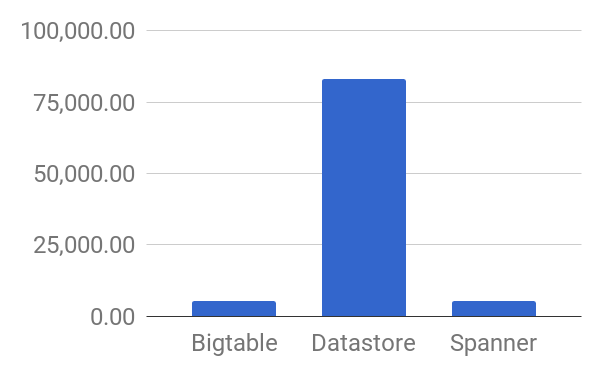
\includegraphics[width=10cm]{load-latency}
	\caption{Latency (\( \mu s\)) for 1000 insert (write) operations}
	\label{load-latency}
\end{figure}
\begin{figure}[ht]
	\centering
	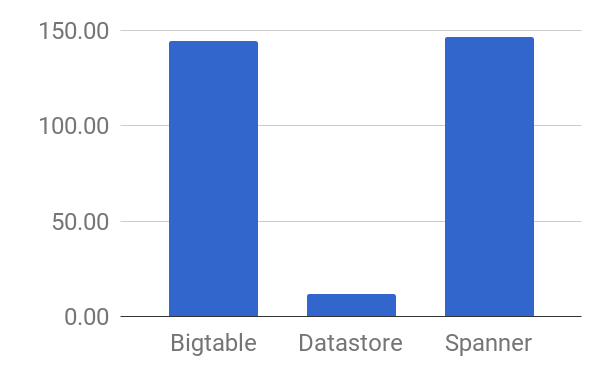
\includegraphics[width=10cm]{load-throughput}
	\caption{Throughput (\(ops/sec\)) for 1000 insert (write) operations}
	\label{load-throughput}
\end{figure}

\subsection{Workloads}

Workload A consists of 1000 operations (500 reads and 500 writes) while workload F consists of 2000 operations (1000 reads, 500 atomic read-modify-write operations and 500 writes). The results of the benchmark in terms of latency on write operations were consistent with the previous loading benchmark results, with Bigtable and Spanner performing significantly better over Datastore (Figure \ref{write-latency}). The latency on write operations showed a clear dominance by Bigtable. 

\begin{wrapfigure}{r}{0.5\textwidth}
	\centering
	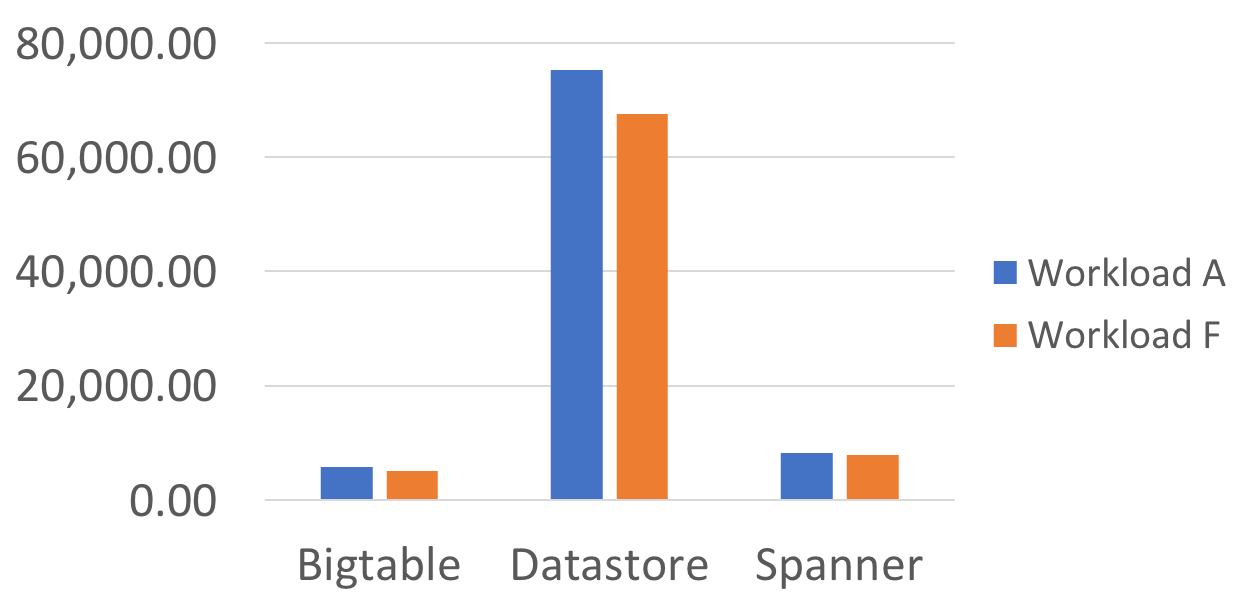
\includegraphics[width=7cm]{write-latency}
	\caption{}
% 	\caption{Write operations latency (\( \mu s\)) for Workload A (500 writes) and Workload B (1000 writes)}
	\label{write-latency}
\end{wrapfigure}

Even though, the difference on read operations latency between Datastore and two other data storages were smaller than with write operations (Figure \ref{read-latency}), Datastore still was more than two times slower than Spanner and more than 4 times slower than Bigtable. The latency results on read-modify-write operations showed a similar trend as read and write operations (Figure \ref{read-modify-write-latency}). 

The overall throughput, again, showed a significant superiority by Bigtable, as indicated in Figure \ref{throughput}. 


\begin{figure}[ht]
	\centering
	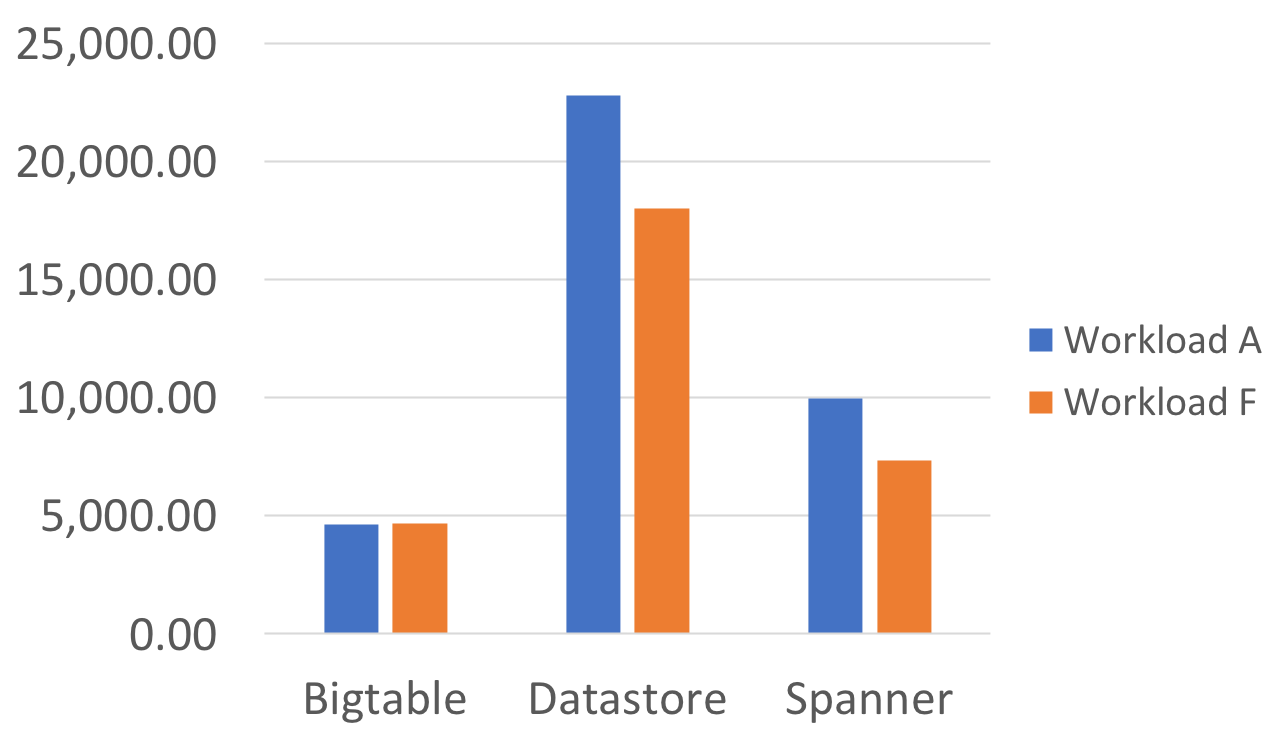
\includegraphics[width=12cm]{read-latency}
	\caption{Read operations latency (\( \mu s\)) for Workload A (500 reads) and Workload B (1000 reads)}
	\label{read-latency}
\end{figure}

\begin{figure}[ht]
	\centering
	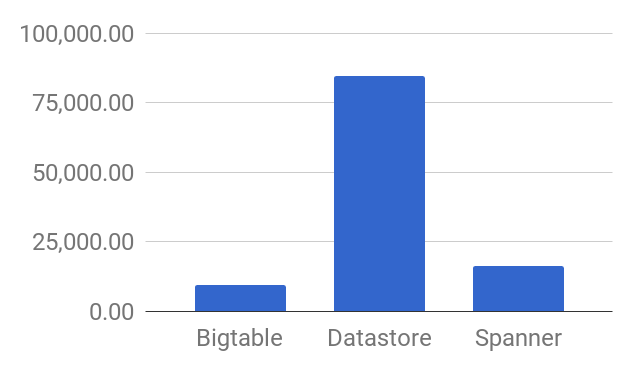
\includegraphics[width=13cm]{read-modify-write-latency}
	\caption{Read-modify-operations latency (\( \mu s\))}
	\label{read-modify-write-latency}
\end{figure}

\begin{figure}[!ht]
	\centering
	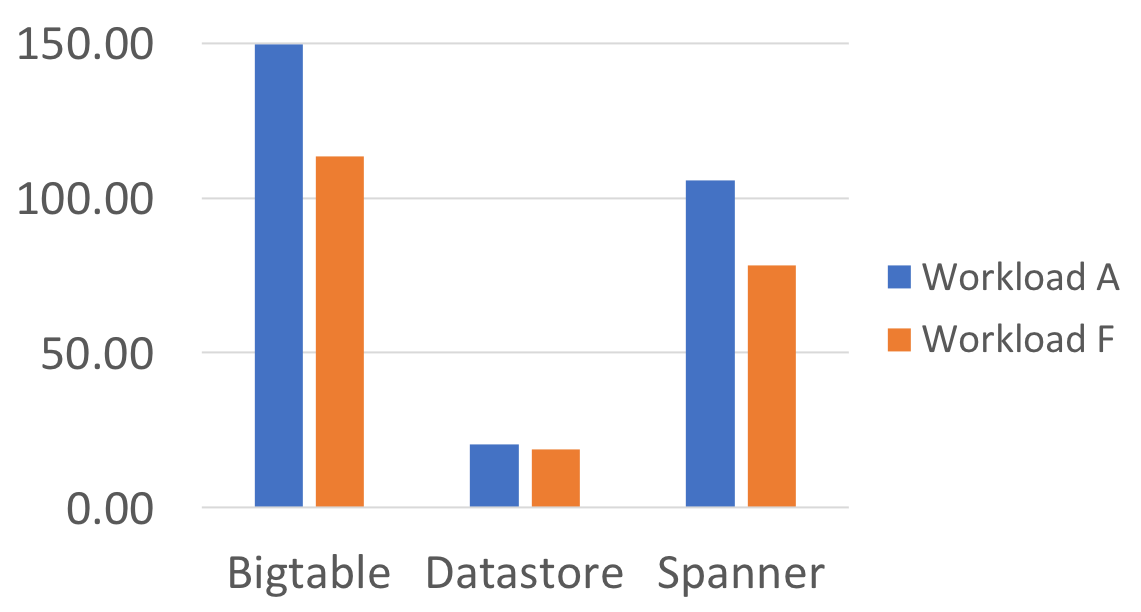
\includegraphics[width=12cm]{throughput}
	\caption{Throughput (\(ops/sec\)) for Workloads A (1000 operations) and Workload B (2000 operations)}
	\label{throughput}
\end{figure}

\subsection{Conclusions}

As Bigtable showed the best results in loading of data and on both of the workloads the benchmarks were run on, and since it provided a strong consistency model, it was selected to be used as a distributed shared memory system for the translation tool.

\section{Reading and writing the contents of Bigtable}

Bigtable uses gRPC client to read and write content using C++ remote function calls. According to gRPC webpage \citep{grpc}, gRPC client application can directly call methods on a server application on a different machine as if it was a local object (similarly to Java RMI). By default gRPC uses protocol buffers, Google's open source language and platform neutral mechanism for serialising structured data. The figure \ref{fig:grpc} visualises communication between gRPC server and client (stub). Bigtable gRPC client is provided through Google APIs repository. In order to simplify the communication with Bigtable table, two functions for putting and getting data to table were implemented, namely put() and get().

\begin{figure}[H]
\centering
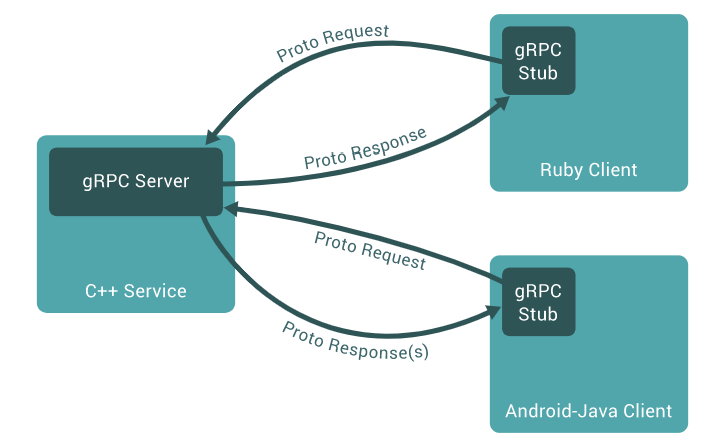
\includegraphics[width=0.9\textwidth]{images/grpc}
\caption{Communication between gRPC server and gRPC stubs (clients) \cite[source:][Guides page]{grpc}}
\label{fig:grpc}
\end{figure}

Put function takes two arguments, 64-bit integer as an address (or key) and 64-bit integer as a value, and does not return anything (see Listing \ref{put}). First, the arguments are casted to string type. Then a new row mutation request is built, by providing full path to the table (including project, instance and table names), row key, family name and column qualifier and value. Family name and column qualifier are constant as we are using Bigtable as key-value store, thus only one column family and qualifier is used. Finally, the row mutation function is called remotely through Bigtable stub and some status information is stored for debugging purposes.

\definecolor{codegreen}{rgb}{0,0.6,0}
\definecolor{codegray}{rgb}{0.5,0.5,0.5}
\definecolor{backcolour}{rgb}{0.95,0.95,0.92}
\lstset{
  mathescape=true,
  literate=
  	{->}{$\rightarrow{}$}{1}
}
\lstdefinestyle{block} {
  language=C++,
  backgroundcolor=\color{backcolour},   
  commentstyle=\color{codegreen},
  keywordstyle=\color{Maroon},
  numberstyle=\tiny\color{codegray},
  stringstyle=\color{magenta},
  basicstyle=\footnotesize,                 
  keepspaces=true,                                           
  tabsize=2,
  captionpos=b
}

\begin{lstlisting}[caption=Writing content to Bigtable using put() function, label=put, style=block]
void put(unsigned long long addr, long long val)  {
	// cast arguments to string type
	string address = std::to_string(addr);
	string value = std::to_string(val);

	// setup the request
	MutateRowRequest req;
	req.set_table_name(tableName);
	req.set_row_key(address);
	auto setCell = req.add_mutations()->mutable_set_cell();
	setCell->set_family_name(familyName);
	setCell->set_column_qualifier(columnQualifier);
	setCell->set_value(value);

	// invoke row mutation on Bigtable
	MutateRowResponse resp;
	grpc::ClientContext clientContext;
	auto status = bigtableStub->MutateRow(&clientContext, req, &resp);
}
\end{lstlisting}

Get function takes an address (or key) with type 64-bit integer as an argument and returns a 64-bit integer value (see Listing \ref{get}). Similarly to put function, the address value is cast to string. A read row request is created by providing the same full path to the table mentioned above and address string is passed as a row key. The call on rows reading function returns a stream, which is read by chunks and appended to the valueStr variable. As all keys in key-value store are assumed to be unique, the nested loops should run at most one time. Before the value is returned, an if statement checks if the given key had the corresponding value in the table and if so, casts the value to 64-bit integer. If no value was found with corresponding key, the function returns 0.

\begin{lstlisting}[caption=Reading content from Bigtable using get() function, label=get, style=block]
long long get(unsigned long long addr) {
	// convert argument to string type
	string address = to_string(addr);

	// setup the request
	ReadRowsRequest req;
	req.set_table_name(tableName);
	req.mutable_rows()->add_row_keys(address);
        
	string valueStr;
	
	// invoke row reading on Bigtable
	auto stream = bigtableStub->ReadRows(&clientContext, req);
	while (stream->Read(&resp)) {
		for (auto& cellChunk : *resp.mutable_chunks()) {
			if (cellChunk.value_size() > 0) {
				valueStr.reserve(cellChunk.value_size());
			}
			valueStr.append(cellChunk.value());
		}
	}
	
	// convert value to 64-bit integer
	long long value = 0;
	if (!valueStr.empty())
		value = stoll(valueStr);
	}
	return value;
}
\end{lstlisting}

\section{Issues encountered}

Even though both gRPC and protobuf (protocol buffers) libraries are developed by Google, some difficulties were encountered while compiling source builds. The errors were made known to the developers \citep{grpc_issue}, but it has slightly stalled the development of the project.

\chapter{Translation tool}

\section{Research on possible solutions}

% Talk about problems with OpenSHMEM and Intel PIN

Having benchmarked and chosen the cloud data store, the next step was to find out ways to invoke write and read operations on Bigtable with data meant to be shared. Three different strategies were identified: library implementation (or source code level solution), binary translation and compiler level solution.

\subsection{Source code level solutions}

The first option for source code level solution would involve creating an application programming interface (API), which includes calls to Bigtable gRPC client with different types of data. This looked like the easiest solution but it would have introduced the requirement for the user to change the source code in order for the tool to work. Moreover, different data types would require different get and put function overloads, thus the search continued on more generic solutions.

Another source code level solution was considered which involved using OpenSHMEM \citep{openshmem}. OpenSHMEM is an open-source partitioned global address space (PGAS) library interface specification. OpenSHMEM implements PGAS by defining remotely accessible data objects (or symmetric data objects) as mechanisms to share information among OpenSMEM processes (also called processing elements) and data objects that are private to each processing element (PE). The interface provides methods to start the OpenSHMEM processing elements in parallel, and communication and synchronization interfaces to access remotely accessible data objects across PEs. The solution using OpenSHMEM involved modifying the API calls for symmetric data objects, changing the storing of shared objects from the symmetric heap (see Figure \ref{fig:openshmem_memory_model}) to Bigtable. Even though this solution would introduce some changes to the user source code, OpenSHMEM is a well-known, broadly used API thus more support would be provided for the user than in the first solution. Unfortunately, OpenSHMEM is more targeted for supercomputers or large high-performance computing clusters with special network setup (i.e. Infiniband network adapters, QsNet interconnect, etc), which is not provided by Google's Compute Engine virtual machines (VMs).

\begin{figure}[H]
\centering
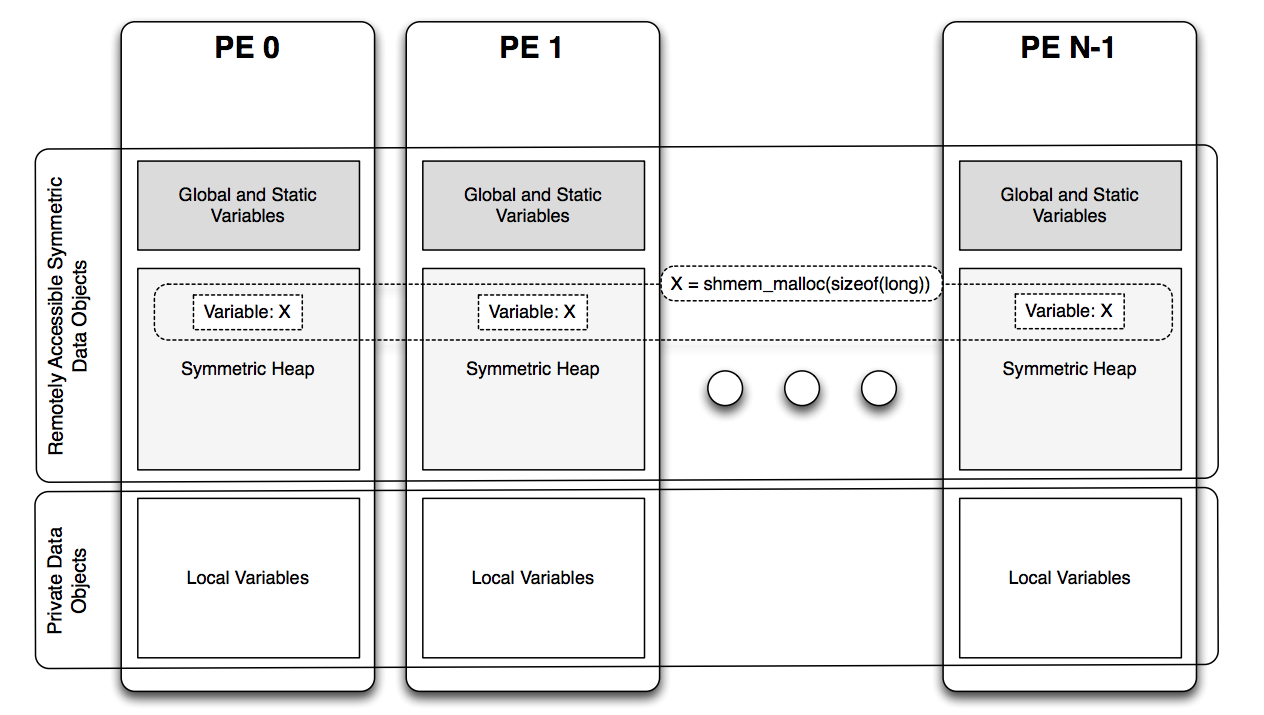
\includegraphics[width=0.9\textwidth]{images/openshmem_memory_model}
\caption{OpenSHMEM Memory Model \cite[source:][]{openshmem_fig}}
\label{fig:openshmem_memory_model}
\end{figure}

\subsection{Compiler level solution}

One way to invoke write and read operations on Bigtable on a compiler level is to customise or create a new compiler, which instead of using load and store instructions for shared memory would call get and put function calls for the Bigtable. Of course, creating a new, industry standard compiler would be too excessive and not feasible in the time span of the project, thus only the customisation of already existing compiler was considered. During the research on this option, a solution using LLVM was discovered. 

\section{LLVM}

% Introduce LLVM

LLVM (Low Level Virtual Machine) is an open source compiler framework for building tools began at the University of Illinois. It supports life-long program analysis and transformation for arbitrary programs. It has an industrial standard compiler (clang/clang++), which has an option to compile C/C++ code to an extensible, strongly typed intermediate representation, namely LLVM IR.

LLVM optimizing compiler, like other industry standard compilers, consists of several components: frontend, optimiser, backend and linker. The important advantage over other compilers is the use of LLVM Bitcode, which consists of a bitstream container format and an encoding of LLVM IR. It provides a clean API boundary separating the compiler frontend and backend, thus making it easier to swap in new frontend and backend components (Figure \ref{fig:llvm}). This is especially useful when developing a new language, as one only needs to create a new frontend component of the compiler and use the provided LLVM optimiser and backend components. 

Moreover, as LLVM project is open-source, users can create their own optimisation or transformation passes. Thus it is possible to create an transformation pass for the optimiser, which would iterate over all of the RISC-like instruction set and translate the appropriate load and store instructions to get and put calls for Bigtable.

LLVM has lots of support and documentation on the Internet. Lots of well-known compilers, like NVIDIA's CUDA Compiler or Microsoft DirectX shader compiler, are based on LLVM. All of these features make LLVM a desirable framework to use for our translation tool.

\begin{figure}[H]
\centering
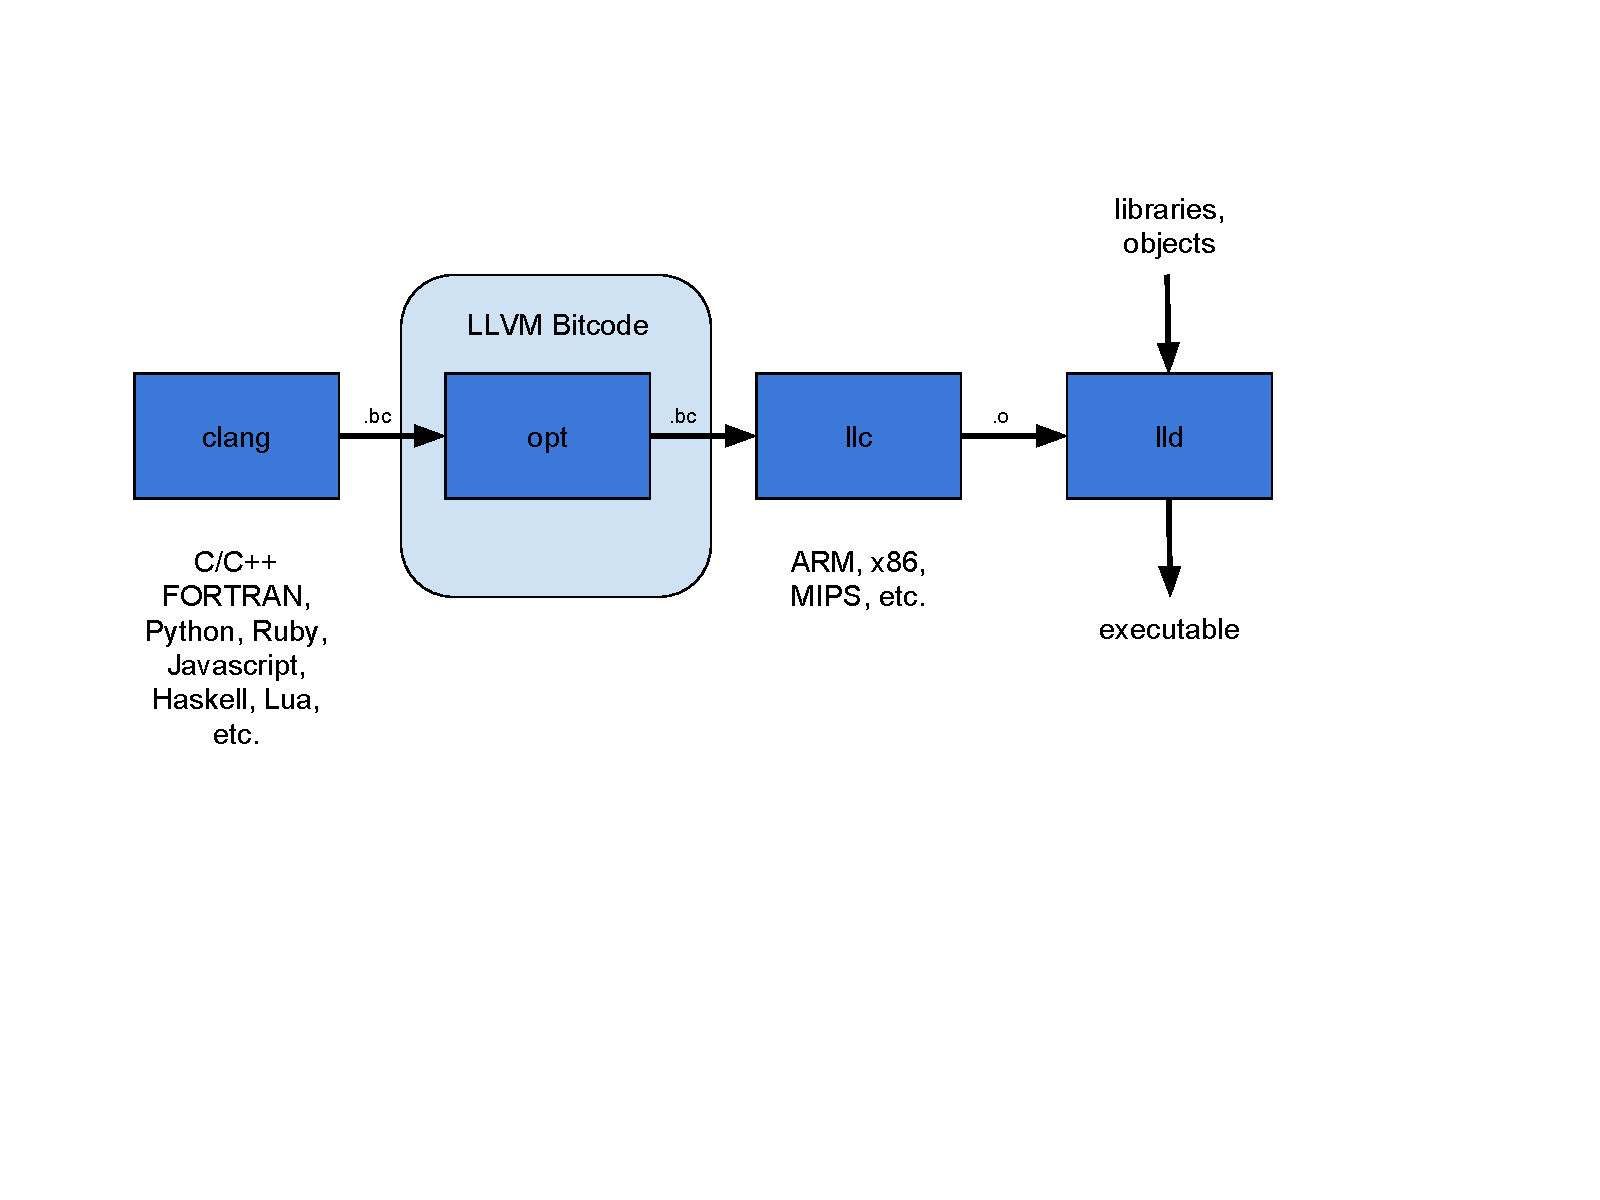
\includegraphics[width=1\textwidth]{images/llvm}
\caption{LLVM compiler architecture}
\label{fig:llvm}
\end{figure}

\section{Architecture}

% Talk about different components involved in translation (user code, get/put functions) and the process of getting instrumented executable

The translation pass tool consists of 4 transitions (see Figure \ref{fig:architecture}). At first, user source code and Bigtable GET/PUT functions are compiled to LLVM IR and combined into a single LLVM Bitcode file. Additional C++ files can be added at this stage if needed later for the LLVM translation pass. After that the code is instrumented by our transformation pass and emits translated LLVM IR into a single LLVM Bitcode file. Then the output is compiled into native machine code and finally linked with gRPC, protobuf and any other relevant libraries to build an executable.

\begin{figure}[H]
\centering
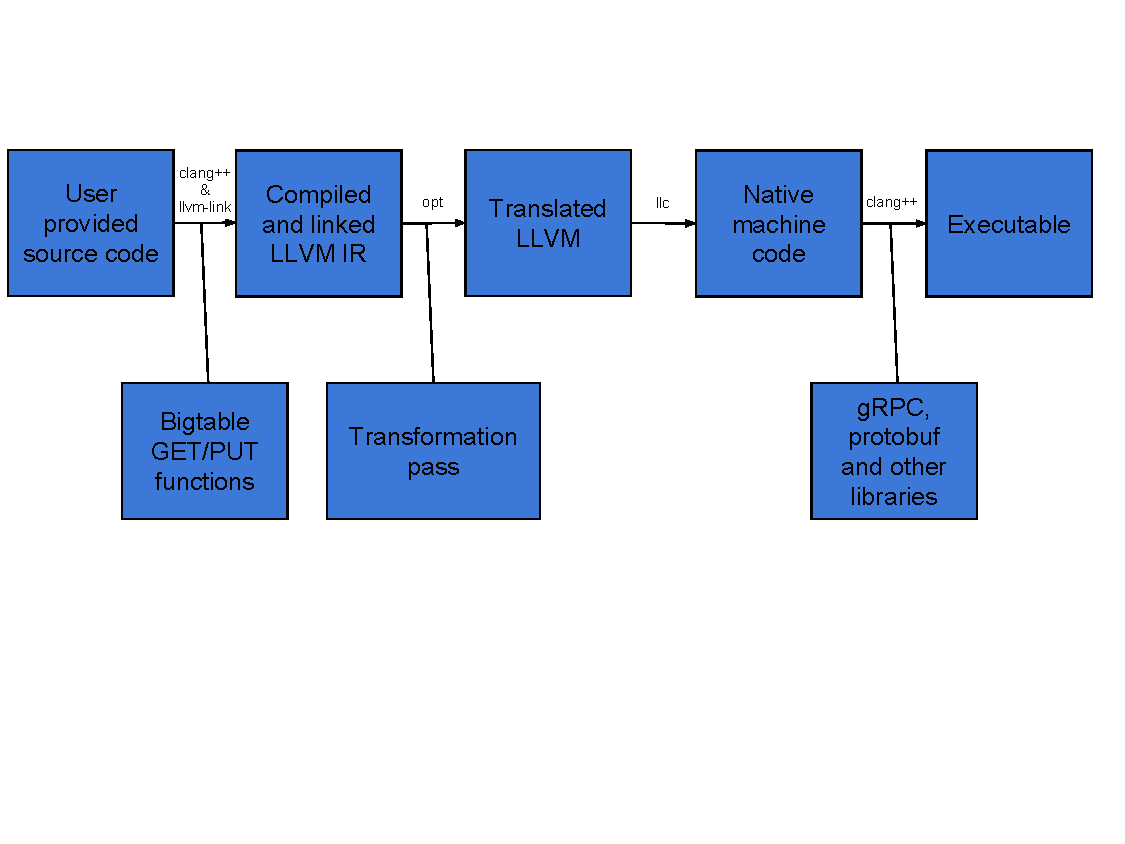
\includegraphics[width=1\textwidth]{images/architecture}
\caption{LLVM solution architecture}
\label{fig:architecture}
\end{figure}

After the preprocessing and compilation of Bigtable GET/PUT functions file, the resulting LLVM Bitcode consists of dozens of gRPC library functions. As we do not want to translate the gRPC load and store instructions, a check was added to the transformation pass, which stops the transformation when the first gRPC function is detected through the iteration. In order for this to work properly, the linking of LLVM Bitcode files in first stage must be done in a strict order: Bigtable GET/PUT functions file must appear after the code that must be translated. This creates a barrier (see Figure \ref{fig:barrier}) between the code that is translated and the code which contains functions to be called translated code (i.e. put and get).

\begin{figure}[H]
\centering
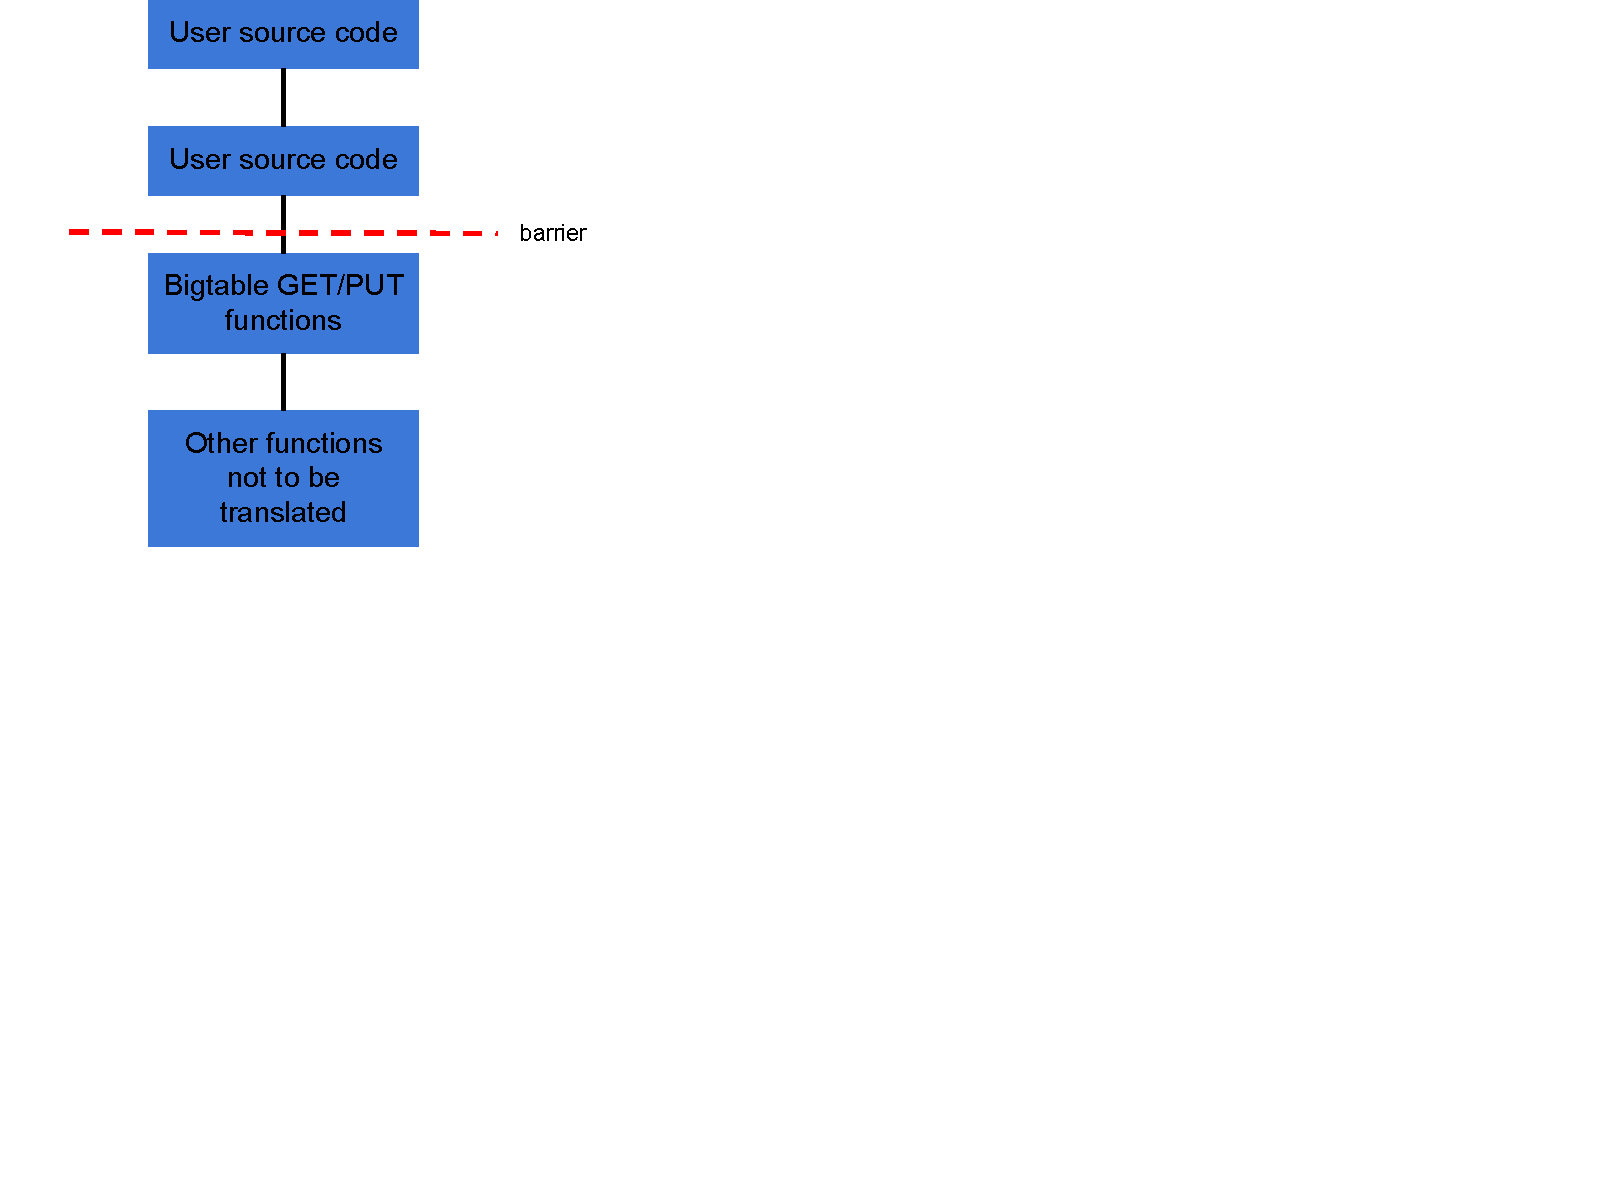
\includegraphics[width=0.5\textwidth]{images/barrier}
\caption{Translation barrier}
\label{fig:barrier}
\end{figure}


\section{LLVM pass}

% Talk about full translation pass
The previously mentioned barrier dividing instrumented and uninstrumented code is implemented by checking if the currently iterated function is from Bigtable GET/PUT functions file. The translation pass iterates over all instructions until the barrier. When the iteration reaches this function, the loop is ended. Moreover, the pass also skips over inline functions with external linkage.  In LLVM, these functions can be detected by hasLinkOnceODRLinkage function call. 

Load and store instructions accept different types of arguments (remember IR is a strongly typed instruction set). For store instructions, the address must have a higher pointer indirection degree than the value. For instance, the corresponding store instruction for \lstinline{int* x = &y} (assuming y is of type integer) would have the address with the type of pointer to pointer to integer and the value with the type of pointer to integer. For load function translations, get function must return the value with the same type as load instruction. Moreover, get and load functions only accepts 64-bit integer arguments, thus sign extension instructions might be needed. This makes the translation of store (and get) instructions more complicated that just replacing one instructions with the others.

Store to put instruction translation starts by converting the address pointer to 64-bit integer with ptrtoint instruction. If the value is of integer type and not 64 bits wide it is sign extended using sext instruction. If the value is of pointer type it is cast to 64-bit integer by ptrtoinst instruction. Otherwise, it is assumed to be 64-bit integer\footnote{Although it might of other type (i.e. struct).}. Finally, both arguments now being of 64-bit\footnote{64-bit integer type for get and put instruction arguments and/or return type was chosen deliberately. This is the maximum biggest type of integer, thus it makes the casting part a bit simpler. For example, if 32-bit integer type was chosen, some values would need to be sign extended while others would need to be truncated.} integer type are given as arguments to put function call. The figure \ref{fig:store_translation} shows a subset of instruction set before and after store instruction translation.

\begin{figure}[H]
\centering
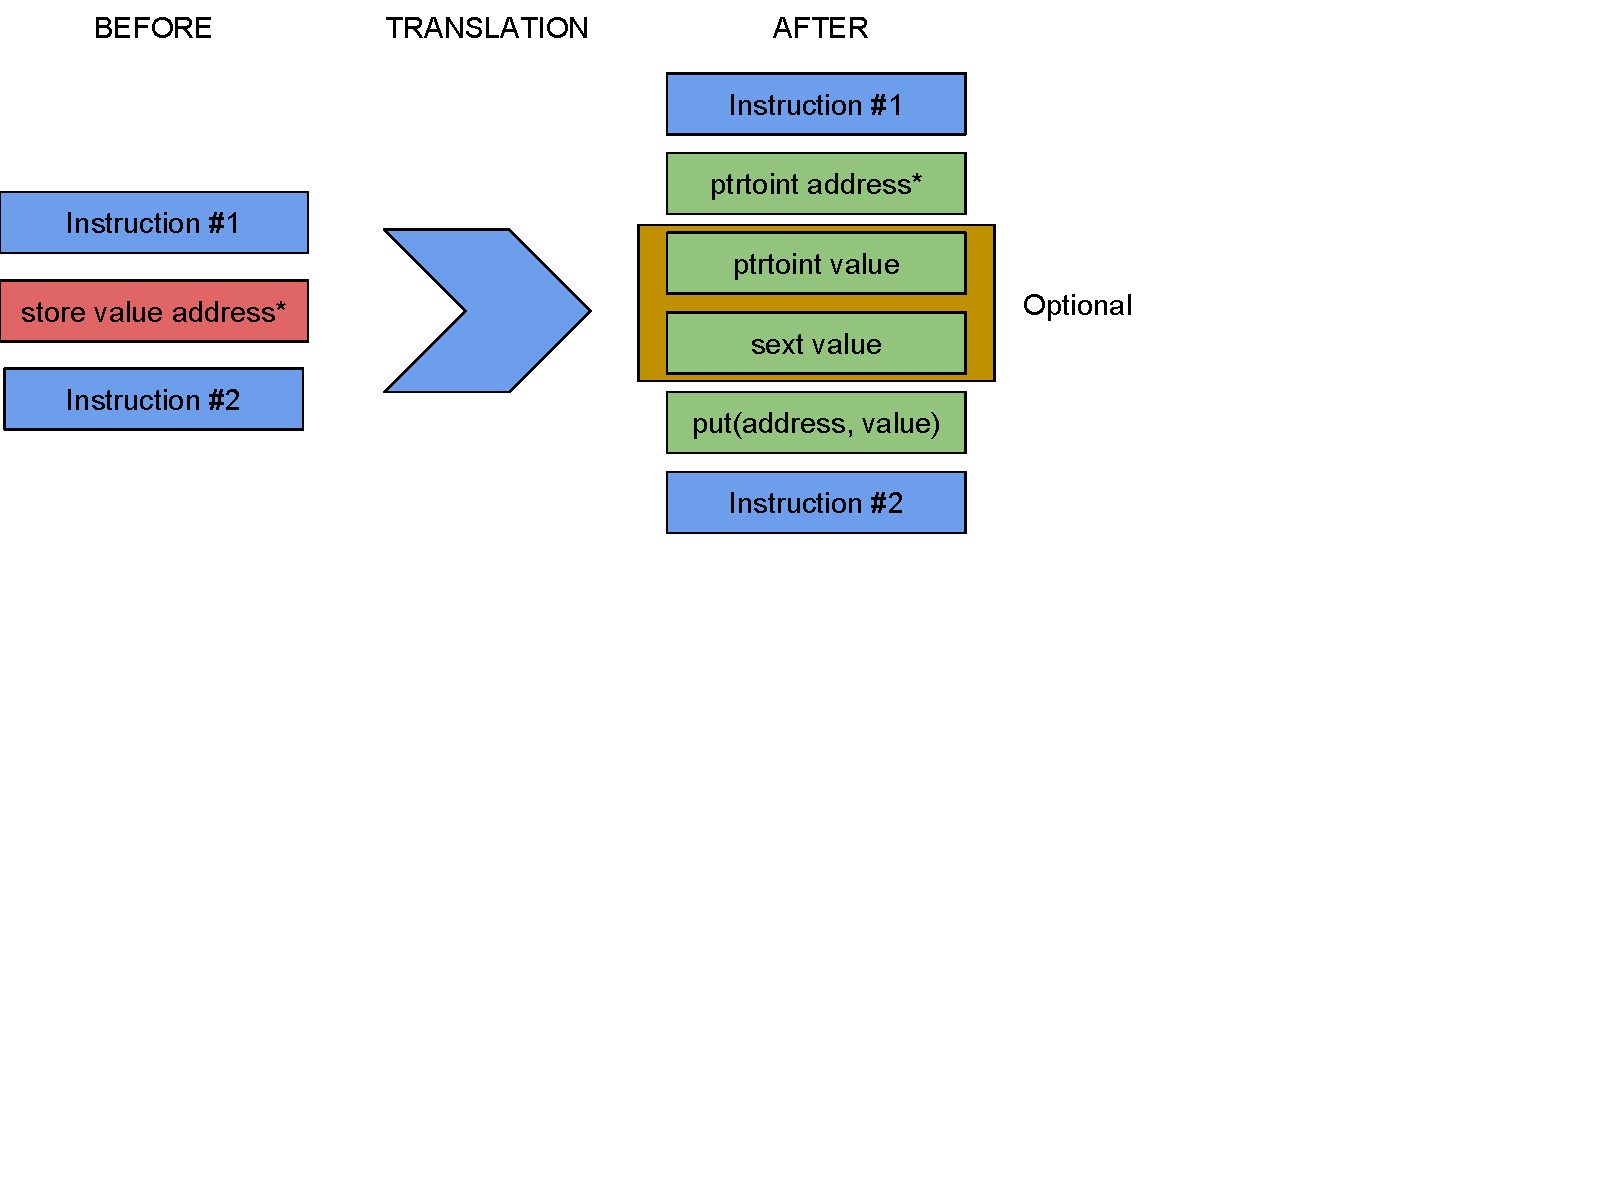
\includegraphics[width=0.8\textwidth]{images/store_translation}
\caption{LLVM instruction set before and after store instruction translation}
\label{fig:store_translation}
\end{figure}

Load instruction translation begins by identifying its return type and pointer indirection degree (only relevant if of pointer type). Similarly to store translation, the address is cast to 64-bit integer using ptrtoint instruction, and passed to get as an argument. As the return type of get function is 64-bit integer, it must be cast to the appropriate type (unless the load instruction actually returns 64-bit integer). If the returned type is integer it is truncated to the expected integer type using trunc instruction. Finally, if the expected returned type is pointer, the resulting value is converted to a pointer type with an appropriate pointer indirection degree (identified at the beginning) with inttoptr instruction. The figure \ref{fig:load_translation} shows a subset of instruction set before and after store instruction translation.

\begin{figure}[H]
\centering
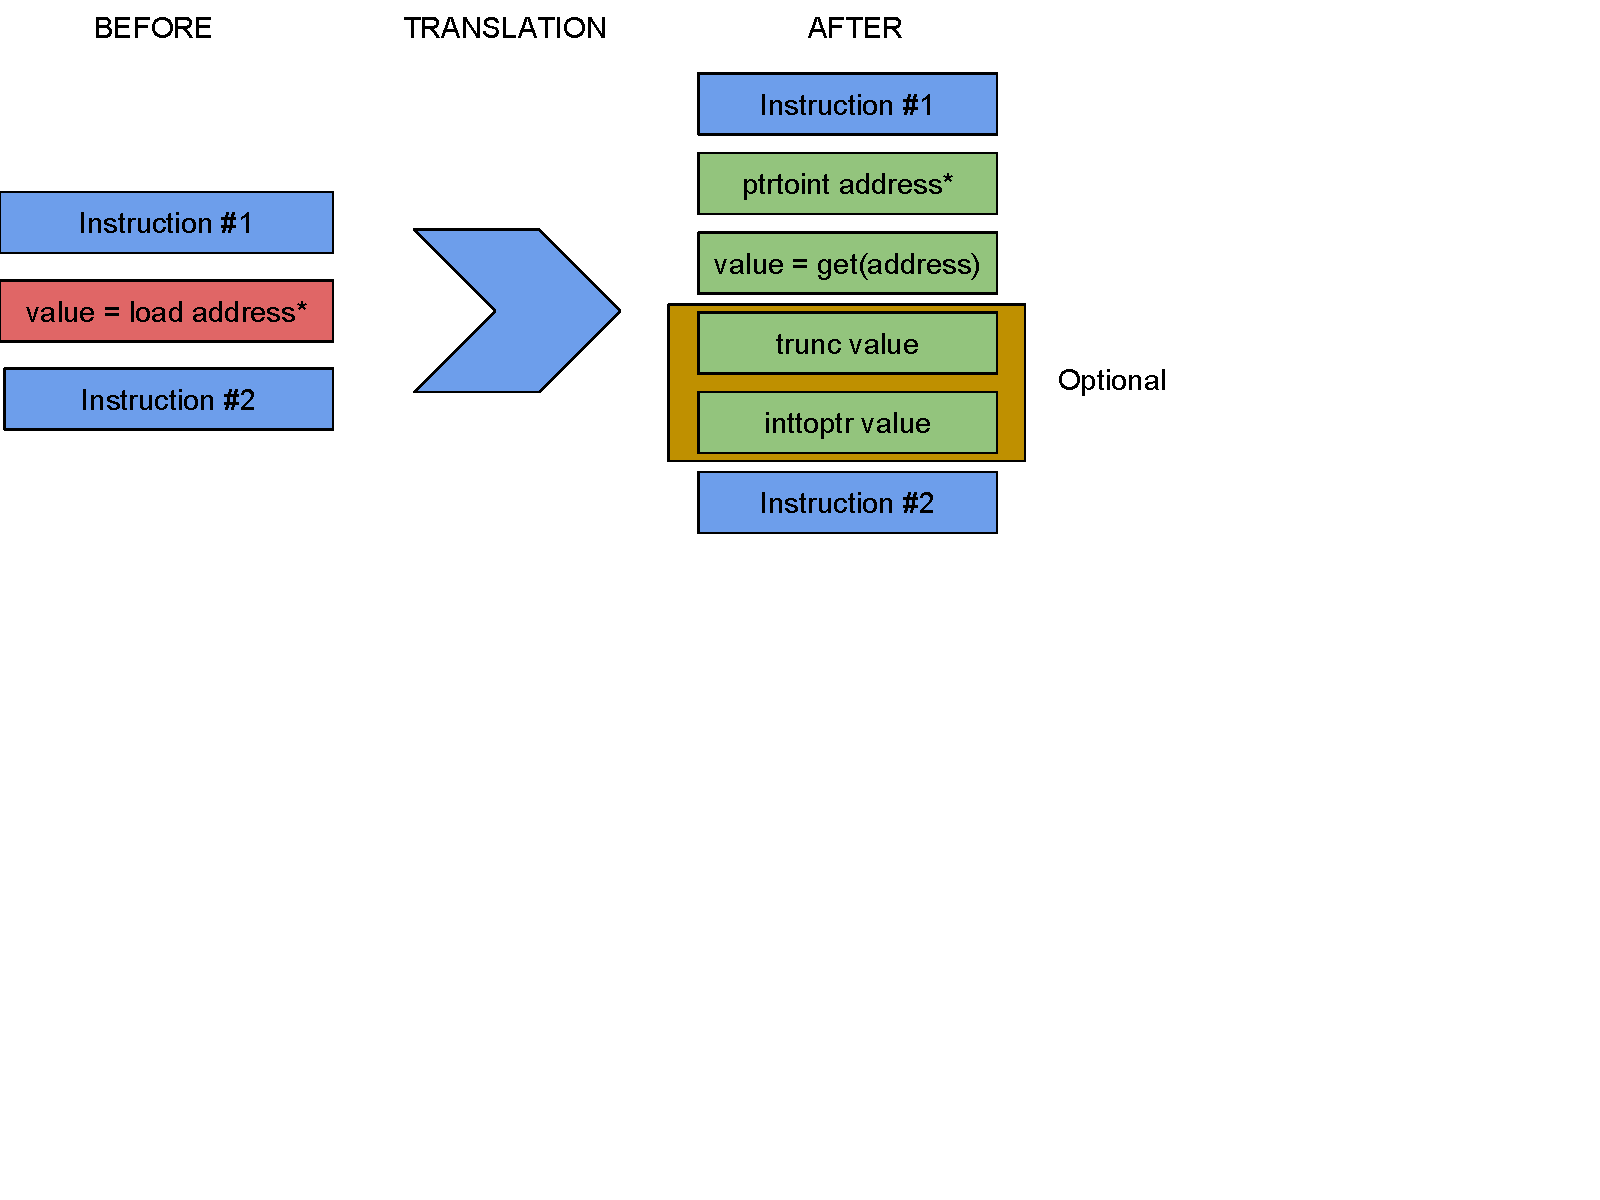
\includegraphics[width=0.8\textwidth]{images/load_translation}
\caption{LLVM instruction set before and after get instruction translation}
\label{fig:load_translation}
\end{figure}


\chapter{Custom heap allocator}

\section{Motivation}

Calls to malloc function allocate virtual memory space. When this allocated virtual memory is "touched" (i.e. load from or stored to), it is mapped to real memory by call to special function of the operating system (i.e. mmap). As translation tool eliminates all loads and stores to memory, the allocated memory is never accessed, thus never really mapped to physical memory. Nevertheless, the allocated memory is left unused on virtual address space. This might cause problems when a program tries to allocate more space than possible on virtual memory. Some operating systems (i.e. Windows or macOS) limit the virtual memory space, thus providing a custom heap allocator, which would reduce the amount of memory allocated on virtual address space, seems beneficial. The proposed solution is a first-fit free-list heap allocator.

\section{Implementation}

The heap allocator implementation was based on Marwan Burelle's malloc tutorial \citep{malloc_tutorial} and adjusted to work on Bigtable. The heap allocator implements four functions: malloc, free, realloc and calloc. All of these functions are counterparts of the Standard C++ Library functions and have the same function definitions.

The allocator keeps a list of meta-data blocks, which contain information about chunks of data allocated with malloc. This lets the memory be reused after it has been released with call to free function. Unlike in tutorial implementation, only meta-data objects are stored on main memory. The actual requested space is allocated on Bigtable. Thus, the implemented custom heap allocator uses two heaps: main memory and Bigtable. The figure \ref{fig:heap_organisation} sketches the memory organisation of two heaps. The structure of meta-data blocks described in the tutorial were adjusted to reflect these changes. Besides storing the size of data block and pointers to other blocks, the meta-data blocks also stores the address of data block on Bigtable.

The main memory heap is managed by the default memory allocator (Standard C++ library provided malloc, free, etc). For the custom heap allocator, it is used as meta-data objects storage.

The heap on Bigtable is implemented as a continuous space of memory with two bounds: the start of the heap and the end point  called the Bigtable break. The start of the heap is initialized on the first call on custom malloc function by calling sbrk function with an increment equal to 0 (this returns the break address on the main memory heap). Thus, the addresses of main memory and Bigtable heap are identical. The end of the heap is managed by set\_bt\_brk function, which was implemented to reflect the behaviour of sbrk function (see Listing \ref{setbtbrk}).

\begin{lstlisting}[caption=set\_bt\_brk function implementation, label=setbtbrk, style=block]
void* set_bt_brk(int incr) {
  // if uninitialised, set to sbrk(0)
  if (current_bt_break == 0) {
    current_bt_break = (uintptr_t) sbrk(0);
    initial_bt_break = current_bt_break;
  }
  uintptr_t old_break = current_bt_break;
  current_bt_break += incr;
  return (void*) old_break;
}
\end{lstlisting}

Of course, another solution could be to allocate both meta-data objects and the actual requested space on the Bigtable, but this would increase the communication costs with Bigtable. As meta-data objects only take up to 40 bytes (on a 64-bit system), the decision was made to store them locally.

\begin{figure}[H]
\centering
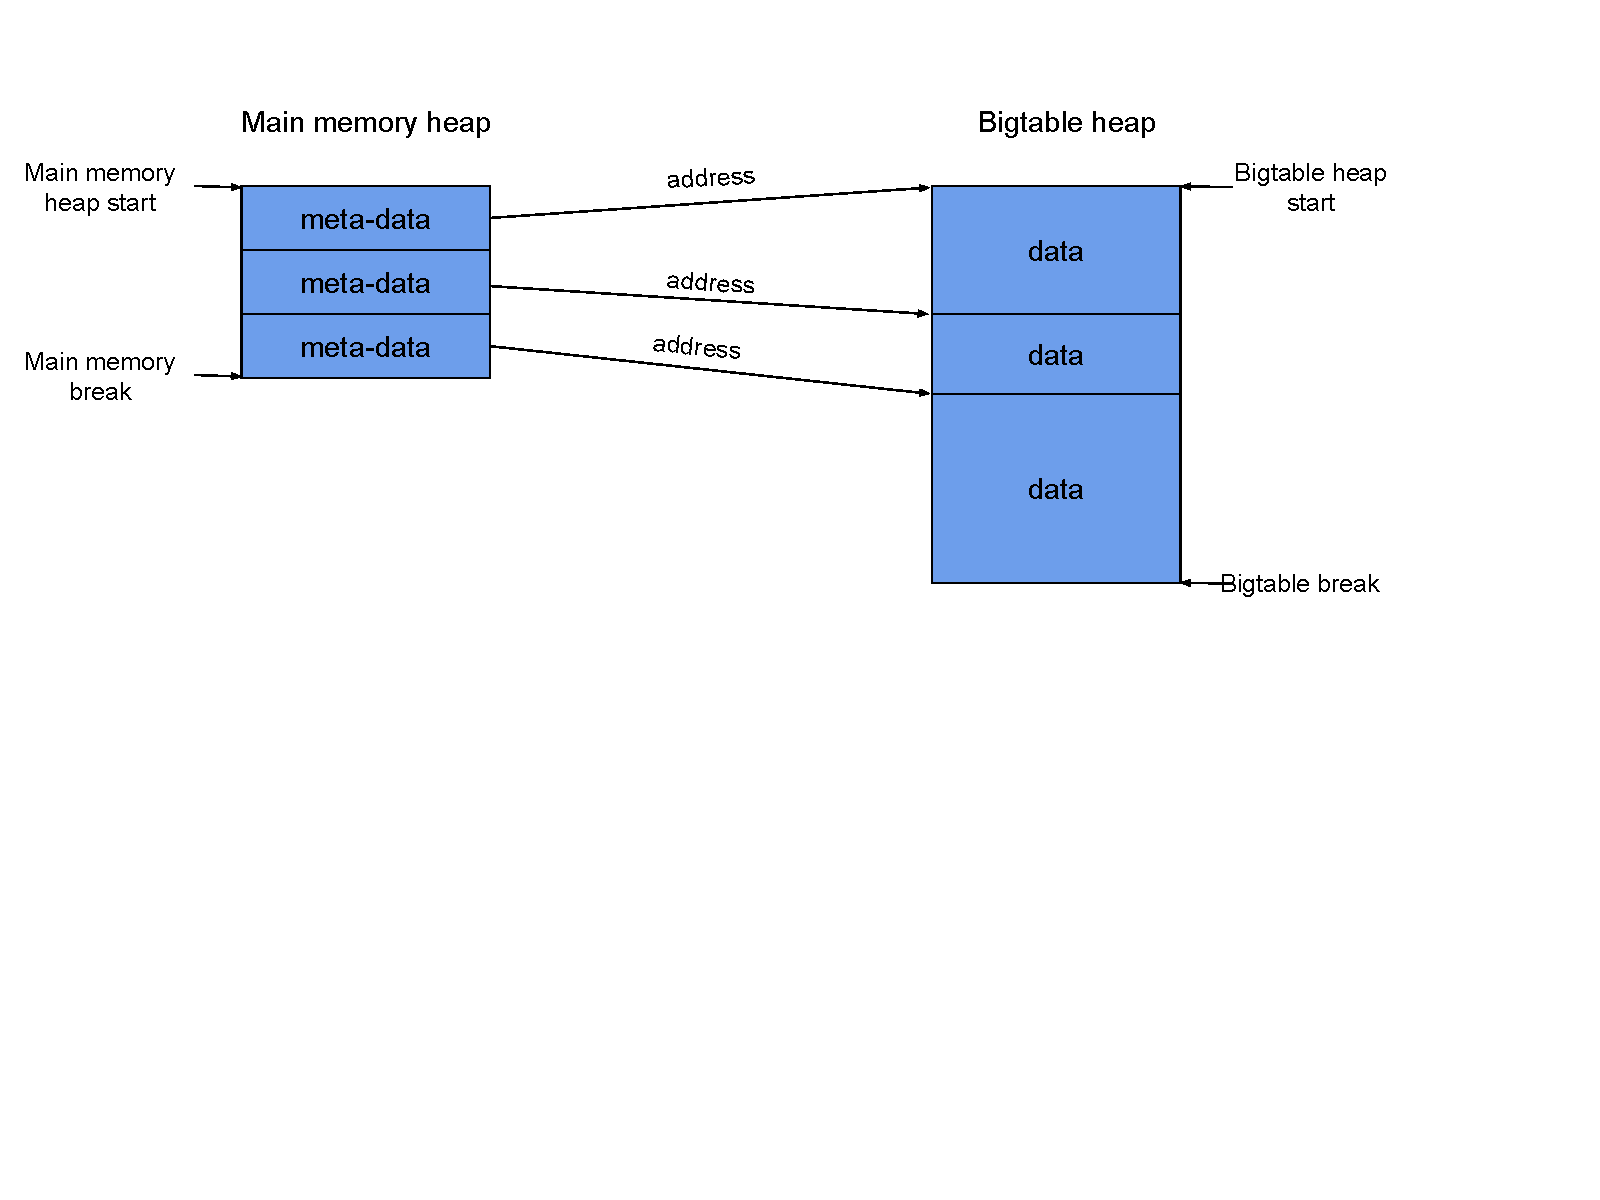
\includegraphics[width=1\textwidth]{images/heap_organisation}
\caption{LLVM instruction set before and after get instruction translation}
\label{fig:heap_organisation}
\end{figure}

Malloc function starts by changing the requested size to be a multiple of 4 to align the pointers by 32 bits. If the heap is not empty (already called malloc() before), the linked list of meta-data blocks is searched for the first free chunk that is wide enough for the request. If such block is found and the difference between the requested size and the size of the block is enough to store a minimum allowed block (32 bytes\footnote{In the popular dlmalloc \citep{leadlmalloc} implementation, the smallest allowed allocation is 32 bytes on a 64-bit system, thus I decided to use the same size in my malloc implementation.}) the block is split into two blocks. The first block is marked as used. If the heap is empty or no existing wide enough block is found, the heap is extended. Finally, the address to the block on Bigtable is returned.

Free function accepts a pointer to heap memory block to be freed and starts by checking if it points to is a valid Bigtable heap address. If it does, the pointer address is used to retrieve the meta-data block. In order to do this efficiently a hash table was introduced to map the data block address to meta-data block. Every time a heap is extended or a block is split, the hash table is updated with a new key-value (address and meta-data block) pair. This is a more efficient solution than iterating over the linked-list of meta-data blocks. After the meta-data block is retrieved, it is freed. If the any of the neighbouring meta-data blocks are free, the blocks are fused into one (to cope with fragmentation). If after the fusion the resulting meta-block is the tail of the linked-list the memory is released. This part was adjusted to decrease the Bigtable break by the size of the block being released. Consequently, the corresponding pair is deleted from the hash table and the meta-data block is freed using default malloc.

Realloc functions accepts two arguments, pointer to existing heap memory block and the new size for the block. If the pointer address is a valid heap address, the meta-data block is fetched using the hash table mentioned above. The size is changed to be aligned with 32-bit pointers. If the requested size is smaller than the original size, the block is split in two. Otherwise, if the next block is free and provide enough space (combined with the original block), the two blocks are fused into one and split if necessary. If none of the options above are true, a new block is allocated with malloc, the old block contents are copied to the new one and, finally, the old block is freed. The block copying procedure was modified to work with Bigtable. The old block values are copied using a combination of GET and PUT function calls to Bigtable (see Listing \ref{copyblock}). Lastly, if the pointer given as an argument to realloc is null, the behaviour is the same as calling malloc with the given size.

\begin{lstlisting}[caption=copy\_block implementation, label=copyblock, style=block]
void copy_block(block src, block dst) {
  int *sdata, *ddata;
  unsigned long long value, *a, b;
  sdata = (int*) src->addr;
  ddata = (int*) dst->addr;
  for (size_t i = 0; i*4 < src->size && i*4 < dst->size; i++) {
    // convert int* to 64-bit integer
    a = (unsigned long long*) &sdata[i];
    b = (unsigned long long) a;  
    value = get(b);
    // convert int* to 64-bit integer
    a = (unsigned long long*) &ddata[i];
    b = (unsigned long long) a;
    put(b, value);
  }
}
\end{lstlisting}

Calloc function accepts an integer representing a number of elements to allocate and an integer representing the size of each element. First, the malloc is called with the product of two arguments. The new block is iterated by 32 bit steps and initialised with 0 values. Again, the implementation was modified to work with Bigtable, using PUT function (see Listing \ref{set0}).

\begin{lstlisting}[caption=new\_block initialisation with zeroes, label=set0, style=block]
  s4 = align4(num * size) >> 2;
  for (i = 0; i < s4; i++) {
    // convert int* to 64-bit integer
    unsigned long long* a = (unsigned long long*) &new_block[i];
    unsigned long long b = (unsigned long long) a;
    put(b, 0ULL);
  }
\end{lstlisting}

For comparison purposes, it was decided to also implement a heap allocator with only a malloc function, without any memory releasing strategy. Heap memory address is incremented with an atomic read-modify-write operation provided by Bigtable. This way the calls to malloc don't have to be synchronised explicitly, as the job is done by atomic calls to Bigtable. 

\section{Consistency on multithreaded programs}

Even though the malloc tutorial was very helpful in implementing a custom heap allocator, it didn't mention anything about allocator consistency on multithreaded programs. The simplest solution to this problem was implemented using a lock. A single mutex was created and the calls to its functions lock and unlock were added to the entry and exit points of malloc, free, realloc and calloc functions. This synchronises the above functions and lets only one thread to make modifications to the heap. This means that no other threads are permitted to do allocations and releases while the other thread is modifying the heap by either of the above functions. Even though this is a correct solution, it is very inefficient. Threads that frequently allocate and release memory form the heap are constantly being blocked or block others threads, essentially making the execution of the program serial.

Another way to solve the thread-safety problem is by allocating a large chunk of memory off the heap to each thread and then managing the space within the thread. However, some threads might not be using all of their allocated memory, which results in poor memory usage efficiency. Moreover, some threads might need more memory than given by default, thus there should be ways to increase the per thread heap memory. Thus, it can be seen that the increase in performance adds additional complexity to the allocator. Clearly, this is a more involved solution and due to a strict time limits for the project it was not implemented. This is one of the areas where the translation tool could be improve in the future work.

\section{Results}

\subsection{Virtual memory usage}

Both heap allocators implemented were tested for virtual memory usage. The figure \ref{fig:malloc_run} shows the linux top command output of memory usage by 4 different runs of an instrumented program. The top left screenshot shows a program run without any heap allocations. It is used as a baseline run to better understand how much memory a simple instrumented program uses. Each of the other 3 program runs malloced 1 gigabyte of memory. Clearly, the programs using the implemented heap allocators solve problem of virtual memory usage, as they do not allocate virtual memory but rather assigns some address space on the Bigtable.

\begin{figure}[H]%
    \centering
    \begin{subfigure}{.4\linewidth}
    	\centering
    	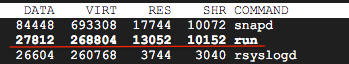
\includegraphics[width=6cm]{images/no_malloc}
	\caption{run without malloc}
    \end{subfigure}
    \hskip2em
    \begin{subfigure}{.4\linewidth}
    	\centering
    	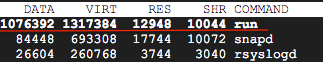
\includegraphics[width=6cm]{images/default_malloc}
	\caption{run with default malloc}
    \end{subfigure}
    \begin{subfigure}{.4\linewidth}
    	\centering
    	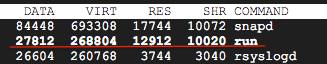
\includegraphics[width=6cm]{images/custom_malloc}
	\caption{run with custom malloc}
    \end{subfigure}
    \hskip2em
    \begin{subfigure}{.4\linewidth}
    	\centering
    	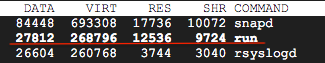
\includegraphics[width=6cm]{images/simple_malloc}
	\caption{run with custom malloc without free}
    \end{subfigure}
    \caption{The Linux top command output of memory usage by 4 different runs of an instrumented program}
    \label{fig:malloc_run}
\end{figure}

\subsection{Performance}

\chapter{Heap memory translator}

\section{Motivation}

It might be preferable to use Bigtable as a storage for only shared data. This way, the concurrency problems with shared memory are handled by the Bigtable, while the rest of the memory is stored locally, thus making the access to it faster. Each thread of the process have its own stack but shares the heap and global variables. As the memory for global variables is already allocated by the frontend of the compiler, it was decided not to translate store and load instructions on these variables. Therefore, a new translator was implemented to instrument only store and load instructions on heap variables. In theory, such translator should work faster than the full memory translator described in Chapter \ref{}, as it translates only a fraction of the existing store and load operations. 

\section{Implementation}

The easiest way to determine if the variable is stored on the heap is to check if its address is inside the heap address space. If the address of the variable is between the start of the heap and the current break of the heap, then we want to store such variable on the Bigtable. Thus, while iterating through instructions we need to check if the address of load or store instruction is inside the heap address space. If it is, we call GET or PUT function on Bigtable and do the similar type casts as in full memory translator. Otherwise, we want to leave the original load or store instruction as is. 

Firstly, the custom heap allocator was extended to have to new functions. The getter functions for heap boundaries. In order to accomplish this, the heap allocator saves the start of the heap on the first call to malloc.

For both store and load instructions the translation starts with calls to get heap boundaries. The address of the translated instruction is cast from pointer type to 64-bit integer and compared using icmp instructions with both heap boundaries. The comparison results are conjoined bitwise and used as a condition for branch instruction. In a case where the bitwise conjunction is equal to 1, the program continues with the instructions for GET or PUT function. Otherwise, the program jumps to the label with the original load or store instructions. If the translated function is load, then a PHI node is added to take on the value corresponding to the input control block (either call to GET function or load instruction). Phi node is an instruction used to select a value depending on the predecessor of the current block.

\begin{figure}[H]%
    \centering
    \begin{subfigure}{.45\linewidth}
    	\centering
    	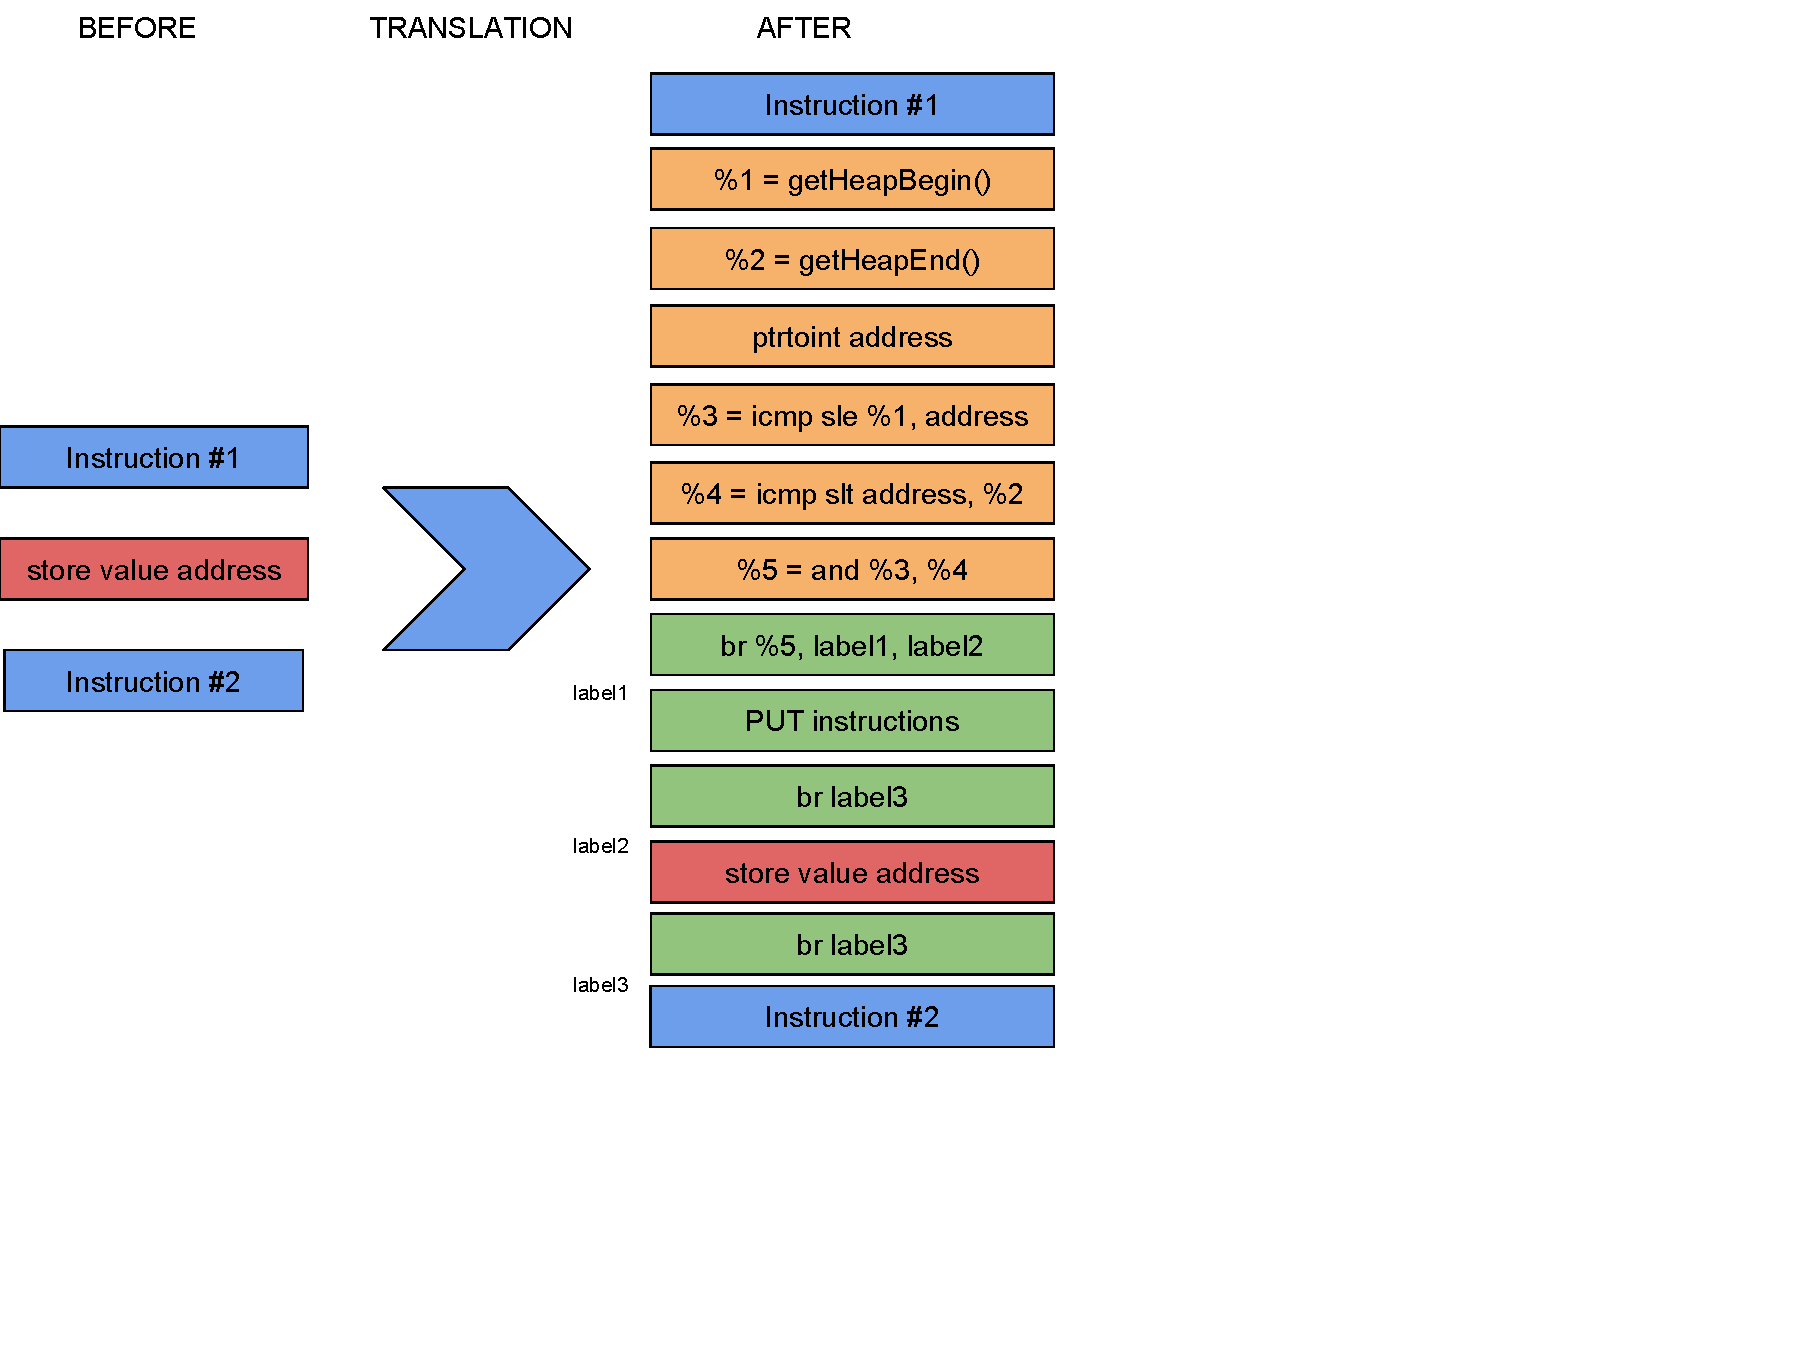
\includegraphics[width=7cm]{images/heap_store_translation}
	\caption{Store instruction translation}
    \end{subfigure}
    \hskip2em
    \begin{subfigure}{.45\linewidth}
    	\centering
    	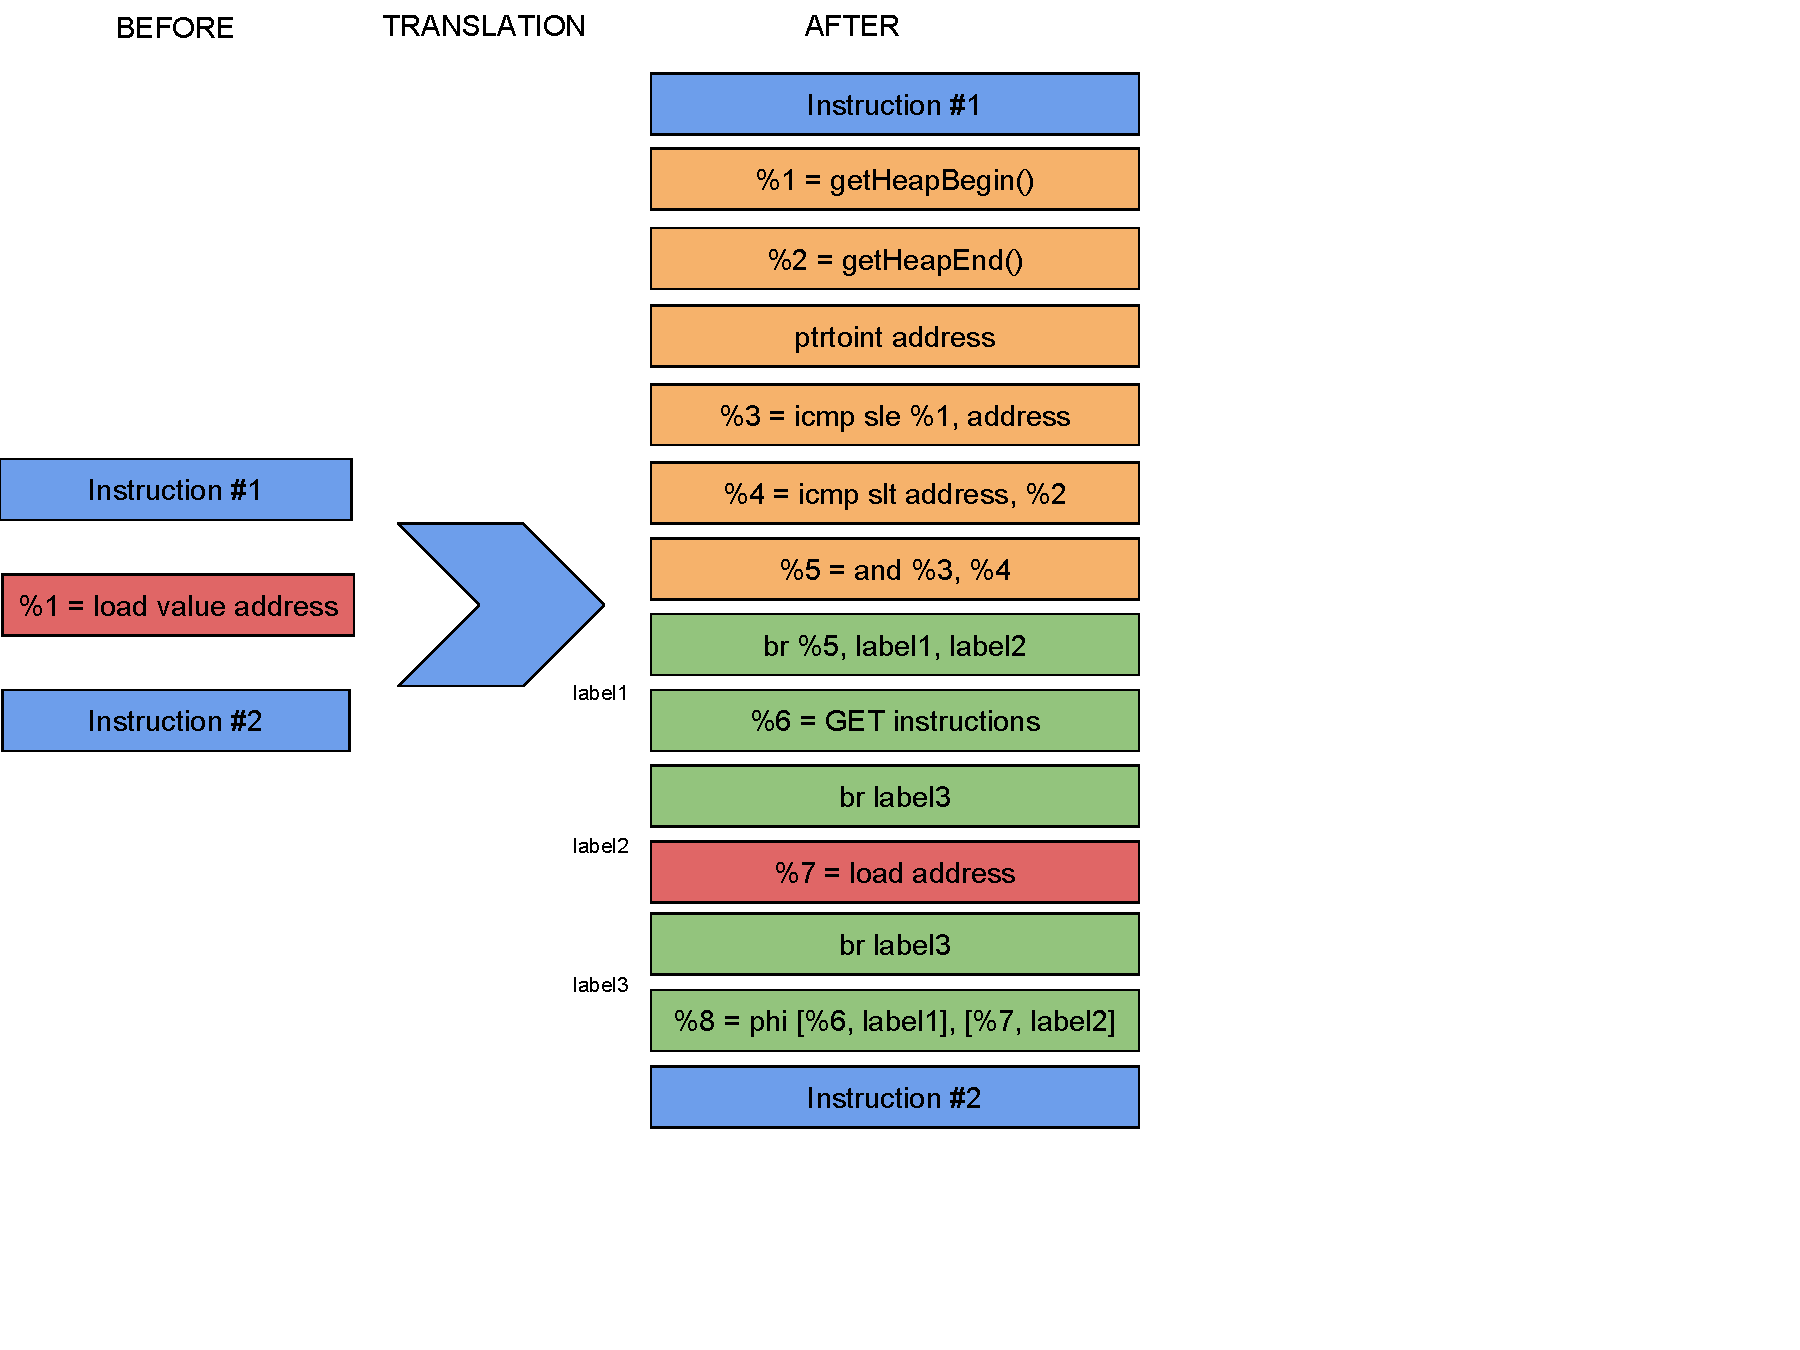
\includegraphics[width=7cm]{images/heap_load_translation}
	\caption{Load instruction translation}
    \end{subfigure}
    \caption{Load and store instruction translation on heap memory translator. Instructions coloured in orange and green are added during translation.}
    \label{fig:heap_translation}
\end{figure}

As seen in figure \ref{fig:heap_translation}, heap memory translation adds a lot of additional instructions. The insertion of instructions is done in several phases. On the first phase, the first six instruction are inserted before (coloured in orange) any load or store instruction. Next, the original basic block the load or store instruction belongs to is split in two and two additional basic blocks for branches are created using SplitBlockAndInsertIfThenElse function. After that the first basic block (label1) is populated by adding a call to GET or PUT function and the casting instructions if needed. The second basic block (label2) is populated with a clone of the original load or store instruction, as the original still exists on the next basic block (label3). Finally, the original store instructions are deleted from the last basic block (label3), while the original load instructions are replaced with phi node instructions.

\chapter{Evaluation}

Even though the translation tool introduced in this paper does not aim to compete on performance with existing technologies, it is still interesting to compare the original  programs with the ones instrumented with the translation tool. Of course, the efficiency of the system which stores and loads all its memory on another machine, however fast the connection between two machines, is not going to compete with the system storing and loading memory situated on the same machine. Nonetheless, performance and other results can be of great value, as they reveal the areas where system could be improved.

% TODO: describe the environment: Google Compute engine VM on the same cluster as Bigtable, etc...

During the testing and evaluation process, it was decided to measure the performance of individual functions rather than the execution of the whole program itself. This decision was taken in order to exclude the time it takes to load the program into memory and prepare it for execution. These measurements are highly depended on the architecture of the machine and the operating system.

\section{Performance}

For the performance benchmarking, wall clock time was used instead of CPU time, as it takes into account the time taken for I/O operations (i.e. calls to Bigtable). All tests are run 100 times and averaged, as the execution time of a single test run fluctuates due to external factors (i.e. OS scheduling, memory usage, etc).

The benchmarking was done using three test functions (source code can be find in Appendix \ref{section:test}), namely stack allocation, heap allocation and parallel producer-consumer problem adapted from Greg Andrews' textbook website \citep{producer-consumer}. The stack allocation test initialises a stack-based 10x10 character matrix with new values. All load and store operations are done on the stack. Similarly, the heap allocation test writes values to heap-allocated 10x10 character matrix. Approximately one of ten load and store instructions are for heap-based accesses. Other, stack-based, memory operations are used for iterating through the matrix. The producer-consumer test uses C's Posix threads (Pthreads) library for thread creation, synchronisation and similar purposes. Also, for this task the time elapsed includes thread creation and join operations. Two threads were used (one for producer and one for consumer operations). The buffer size was set to 1, while, in total, 50 integers were produced/consumed by the algorithm. A simple adjustment was made to allocate buffer on the heap in order to have at least one GET or PUT function call on the function translated with heap translator.

As expected the original program with load and store operations on memory situated on the same machine worked efficiently. The producer-consumer took more than a thousand times longer than the other two tests, as the execution time was capped by thread creation and synchronisation time. The stack allocation and heap allocation tests translated with full memory translator took six orders of magnitude longer to execute. This immense increase in time is due to the introduced communication costs to access memory on Bigtable. The producer-consumer problem took half as long to execute, yet the increment from the original code execution time was enormous. Unsurprisingly, the program translated with heap translator showed a huge improvement over the fully translated program in stack allocation test. The improvement is quite clear as none of the load or store instructions are translated, as only heap memory instructions are translated with heap translator. The slow down compared to the original program can be explained by the increase in instruction count of the program (more detailed analysis on this measure provided in the next section). The heap allocation test on the program transformed by heap translator performs 10 times better than to corresponding test instrumented by full memory translator. Heap allocation test skips all stack-based GET and PUT calls on Bigtable and instead stores these variables locally. The test is capped by the time taken to execute 100 put operations on Bigtable. Producer-consumer test again saves some time on load and store instructions on stack variables. The actual results gathered from benchmarking are shown in table \ref{table:performance}.

\begin{table}[h]
\centering
\begin{tabular}{ c | c c c }
Test & Original & Fully translated & Heap translated \\
\hline
Stack allocation & 0.411 & 2,798,858 & 3 \\
Heap allocation & 0.521 & 2,209,032 & 284,047 \\
Producer-Consumer & 963.717 & 1,272,932 & 295,448
\end{tabular}
\caption{Time taken to execute each function in microseconds ($\mu s$)}
\label{table:performance}
\end{table}

Overall, it can be seen that the heap translation tool is an improvement over full memory translator but it is still makes the functions run hundreds (producer-consumer test) and even hundreds of thousands (heap allocation test) times slower.

\section{Instruction count}

Instruction count was done using an implemented instruction count pass on test program (see Appendix \ref{section:test}), which includes the performance tests mentioned in the section above. The pass iterates over the functions of the program and prints the count of instructions per function and the total number of instructions in the program. To clarify, this is a static count of the instructions and does not account for how many times any particular instruction can be executed on the runtime. Moreover, the instruction count does not include the instructions from shared libraries and their functions.

\begin{figure}[H]
\centering
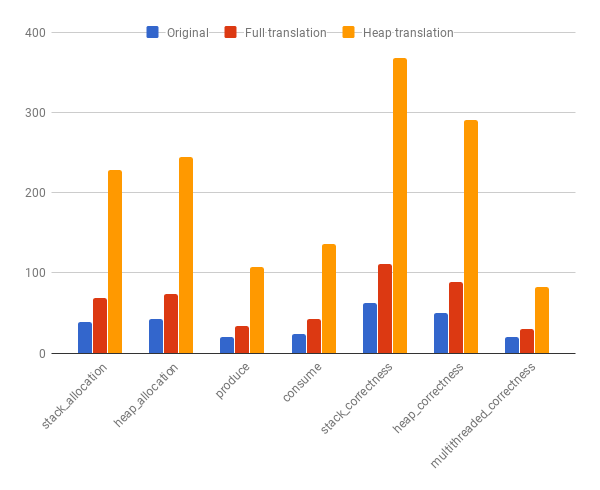
\includegraphics[width=1\textwidth]{images/instruction_count}
\caption{LLVM instruction counts for different functions.}
\label{fig:instruction_count}
\end{figure}

The original program shows the smallest instruction count on every function and works as a baseline for the programs instrumented with the implemented translation tools. The total instruction count for a program translated with full memory translator increased from 571, achieved by the original program, to 761, which shows a 33 percent growth. On average, each function, on average, increased by 27 instructions. The inflation is a result of translating one load/store instruction with a call to get/put function plus 1-3 casting instructions. A much more substantial growth can be seen in functions translated by heap memory translator. The total amount of instructions is 209 percent higher than in the original program, increasing from 571 to 1768 instructions. Each function, on average, increased by 171 instructions. This can be explained by the additional control flow added to distinguish between memory access to heap and stack variables. The translation adds 9 to 14 instructions per store/load instruction.

Overall, the translation adds a lot of additional instructions. This does not necessarily convert to lower performance of the program (as can be seen by heap translation example with stack allocation test in the previous chapter) and is a much smaller problem then the huge increases in execution time, yet it is definitely a measure which could be improved.

\chapter{Conclusions}

\section{Overview}

This report has introduced a translation tool (with two of its variations), which provides a way to run programs requiring amount of memory that cannot be served by user machine. The translation tool instruments the program by changing all load and store operations to get and put calls on Bigtable, respectively. Additionally, a heap memory translation tool was implemented to translate memory which is shared among threads. This tool can be seen as a step towards an instrument which could expose Bigtable as distributed shared memory to multiple machines (more on that in the next section). The report has also showed that the performance of the instrumented programs are orders of magnitude worse than the original programs. This is mainly caused by the communication costs introduced by calls to Bigtable. Overall, even though the translation tools implemented make the programs run extremely slow, they can be successfully used to overcome lack-of-memory problems.

\section{Future work}

There are many opportunities for extending the work done and improving the tools for load and store instruction translation. Some of these directions are presented in this section.

One major area of future work might be to implement a separate front-end compiler. The important feature of the compiler would be to prevent global variables from being allocated space on main memory. Instead they would be stored on Bigtable. This could also be done with stack variables.

Another major improvement would be to introduce synchronisation through Bigtable between multiple instrumented programs running on different machines. The synchronisation could be achieved by using locks, barriers and other primitives. Bigtable provides an atomic fetch-and-add operation, which can be used as a generalised test-and-set operation, thus it is possible to implement the synchronisation primitives.

There might also be a way to slightly improve the performance of the translated programs by introducing caches. They would store small amount of memory in them and be updated on put operations to Bigtable. Combined with the synchronisation primitives and an appropriate cache coherence protocol the updates would let expose Bigtable as distributed shared memory.

Other possible improvements on the tool:
\begin{itemize}
\item
Implement all memory functions provided by C/C++ standard libraries. This task was already started by implementing a memcpy function, which is used to make copies of struct type variables. The original C/C++ standard library functions use load and store instructions. These must be change to get and put operations on Bigtable. This is quite important as users might need to use these functions in their programs.
\item
better support for getting and putting structured data to Bigtable. For instance, C++ standard library class Tuple is represented as a literal struct type (\{i32, *i32\}). Load and store instructions provided by LLVM cope with these type of structures, yet the control flow created by the translation tries to cast the type into 64-bit integer and loses parts of data (32 most significant bits) on the cast back. 
\item
A get and put function overloads should be provided for ConstantFP (floating point) type in order to correctly store floating point values on Bigtable.
\end{itemize}

These extensions could make the translation tools more practical and attractive to potential users.

% use the following and \citep{} as above if you use BibTeX
% otherwise generate bibtem entries
\bibliographystyle{plainnat}
\bibliography{mybibfile}

\appendix
\chapter{Test program}
\label{section:test}

\begin{lstlisting}[style=block]
void test_stack_allocation(char matrix[][M_Y]) {
  for (int i = 0; i < M_X; i++) {
    for (int j = 0; j < M_Y; j++) {
      matrix[i][j] = (i * M_Y + j) % 128;
    }
  }
}

char *test_heap_allocation() {
  for (int i = 0; i < M_X; i++) {
    for (int j = 0; j < M_Y; j++) {
      *(heap_matrix + i * M_Y + j) = (i * M_Y + j) % 128;
    }
  }
}

void *produce(void *arg) {
  for (int i = 1; i <= N; i++) {
    sem_wait(&empty);
    *data = i;
    sem_post(&full);
  }
  return NULL;
}

void *consume(void *arg) {
  int total = 0;
  for (int i = 0; i < N; i++) {
    sem_wait(&full);
    total += *data;
    sem_post(&empty);
  }
  return NULL;
}

bool test_stack_correctness(char matrix[][M_Y]) {
  for (int i = 0; i < M_X; i++) {
    for (int j = 0; j < M_Y; j++) {
      if (matrix[i][j] != (i * M_Y + j) % 128) {
        cout << i * M_Y + j << "  " << matrix[i][j] << endl;
        return false;
      }
    }
  }
  return true;
}

bool test_heap_correctness(char *matrix) {
  bool correct = true;
  for (int i = 0; i < M_X; i++) {
    for (int j = 0; j < M_Y; j++) {
      if (*(matrix + i * M_Y + j) != (i * M_Y + j) % 128) {
        correct = false;
      }
    }
  }
  free(matrix);
  return correct;
}

void *test_multithreaded_correctness(void *arg) {
  for (int i = 0; i < N; i++) {
    sem_wait(&lock);
    target++;
    sem_post(&lock);
  }
  return NULL;
}
\end{lstlisting}

\end{document}
